% **************************************************************************************************************
% A Classic Thesis Style
% An Homage to The Elements of Typographic Style
%
% Copyright (C) 2015 André Miede http://www.miede.de
%
% If you like the style then I would appreciate a postcard. My address 
% can be found in the file ClassicThesis.pdf. A collection of the 
% postcards I received so far is available online at 
% http://postcards.miede.de
%
% License:
% This program is free software; you can redistribute it and/or modify
% it under the terms of the GNU General Public License as published by
% the Free Software Foundation; either version 2 of the License, or
% (at your option) any later version.
%
% This program is distributed in the hope that it will be useful,
% but WITHOUT ANY WARRANTY; without even the implied warranty of
% MERCHANTABILITY or FITNESS FOR A PARTICULAR PURPOSE.  See the
% GNU General Public License for more details.
%
% You should have received a copy of the GNU General Public License
% along with this program; see the file COPYING.  If not, write to
% the Free Software Foundation, Inc., 59 Temple Place - Suite 330,
% Boston, MA 02111-1307, USA.
%
% **************************************************************************************************************
\RequirePackage{fix-cm} % fix some latex issues see: http://texdoc.net/texmf-dist/doc/latex/base/fixltx2e.pdf
\documentclass[ twoside,openright,titlepage,numbers=noenddot,headinclude,%1headlines,% letterpaper a4paper
                footinclude=true,cleardoublepage=empty,abstractoff, % <--- obsolete, remove (todo)
                BCOR=5mm,paper=a4,fontsize=11pt,%11pt,a4paper,%
                ngerman,american,%
                ]{scrreprt}

%********************************************************************
% Note: Make all your adjustments in here
%*******************************************************
% ****************************************************************************************************
% classicthesis-config.tex 
% formerly known as loadpackages.sty, classicthesis-ldpkg.sty, and classicthesis-preamble.sty 
% Use it at the beginning of your ClassicThesis.tex, or as a LaTeX Preamble 
% in your ClassicThesis.{tex,lyx} with % ****************************************************************************************************
% classicthesis-config.tex 
% formerly known as loadpackages.sty, classicthesis-ldpkg.sty, and classicthesis-preamble.sty 
% Use it at the beginning of your ClassicThesis.tex, or as a LaTeX Preamble 
% in your ClassicThesis.{tex,lyx} with % ****************************************************************************************************
% classicthesis-config.tex 
% formerly known as loadpackages.sty, classicthesis-ldpkg.sty, and classicthesis-preamble.sty 
% Use it at the beginning of your ClassicThesis.tex, or as a LaTeX Preamble 
% in your ClassicThesis.{tex,lyx} with \input{classicthesis-config}
% ****************************************************************************************************  
% If you like the classicthesis, then I would appreciate a postcard. 
% My address can be found in the file ClassicThesis.pdf. A collection 
% of the postcards I received so far is available online at 
% http://postcards.miede.de
% ****************************************************************************************************


% ****************************************************************************************************
% 0. Set the encoding of your files. UTF-8 is the only sensible encoding nowadays. If you can't read
% äöüßáéçèê∂åëæƒÏ€ then change the encoding setting in your editor, not the line below. If your editor
% does not support utf8 use another editor!
% ****************************************************************************************************
\PassOptionsToPackage{utf8}{inputenc}
	\usepackage{inputenc}

% ****************************************************************************************************
% 1. Configure classicthesis for your needs here, e.g., remove "drafting" below 
% in order to deactivate the time-stamp on the pages
% ****************************************************************************************************
\PassOptionsToPackage{eulerchapternumbers,listings,drafting,%
					 pdfspacing,%floatperchapter,%linedheaders,%
					 subfig,beramono,eulermath,parts}{classicthesis}                                        
% ********************************************************************
% Available options for classicthesis.sty 
% (see ClassicThesis.pdf for more information):
% drafting
% parts nochapters linedheaders
% eulerchapternumbers beramono eulermath pdfspacing minionprospacing
% tocaligned dottedtoc manychapters
% listings floatperchapter subfig
% ********************************************************************


% ****************************************************************************************************
% 2. Personal data and user ad-hoc commands
% ****************************************************************************************************
\newcommand{\myTitle}{A Classic Thesis Style\xspace}
\newcommand{\mySubtitle}{An Homage to The Elements of Typographic Style\xspace}
\newcommand{\myDegree}{Doktor-Ingenieur (Dr.-Ing.)\xspace}
\newcommand{\myName}{André Miede\xspace}
\newcommand{\myProf}{Put name here\xspace}
\newcommand{\myOtherProf}{Put name here\xspace}
\newcommand{\mySupervisor}{Put name here\xspace}
\newcommand{\myFaculty}{Put data here\xspace}
\newcommand{\myDepartment}{Put data here\xspace}
\newcommand{\myUni}{Put data here\xspace}
\newcommand{\myLocation}{Saarbrücken\xspace}
\newcommand{\myTime}{September 2015\xspace}
\newcommand{\myVersion}{version 4.2\xspace}

% ********************************************************************
% Setup, finetuning, and useful commands
% ********************************************************************
\newcounter{dummy} % necessary for correct hyperlinks (to index, bib, etc.)
\newlength{\abcd} % for ab..z string length calculation
\providecommand{\mLyX}{L\kern-.1667em\lower.25em\hbox{Y}\kern-.125emX\@}
\newcommand{\ie}{i.\,e.}
\newcommand{\Ie}{I.\,e.}
\newcommand{\eg}{e.\,g.}
\newcommand{\Eg}{E.\,g.} 
% ****************************************************************************************************


% ****************************************************************************************************
% 3. Loading some handy packages
% ****************************************************************************************************
% ******************************************************************** 
% Packages with options that might require adjustments
% ******************************************************************** 
%\PassOptionsToPackage{ngerman,american}{babel}   % change this to your language(s)
% Spanish languages need extra options in order to work with this template
%\PassOptionsToPackage{spanish,es-lcroman}{babel}
	\usepackage{babel}                  

\usepackage{csquotes}
\PassOptionsToPackage{%
    %backend=biber, %instead of bibtex
	backend=bibtex8,bibencoding=ascii,%
	language=auto,%
	style=numeric-comp,%
    %style=authoryear-comp, % Author 1999, 2010
    %bibstyle=authoryear,dashed=false, % dashed: substitute rep. author with ---
    sorting=nyt, % name, year, title
    maxbibnames=10, % default: 3, et al.
    %backref=true,%
    natbib=true % natbib compatibility mode (\citep and \citet still work)
}{biblatex}
    \usepackage{biblatex}

\PassOptionsToPackage{fleqn}{amsmath}       % math environments and more by the AMS 
    \usepackage{amsmath}

% ******************************************************************** 
% General useful packages
% ******************************************************************** 
\PassOptionsToPackage{T1}{fontenc} % T2A for cyrillics
    \usepackage{fontenc}     
\usepackage{textcomp} % fix warning with missing font shapes
\usepackage{scrhack} % fix warnings when using KOMA with listings package          
\usepackage{xspace} % to get the spacing after macros right  
\usepackage{mparhack} % get marginpar right
\usepackage{fixltx2e} % fixes some LaTeX stuff --> since 2015 in the LaTeX kernel (see below)
%\usepackage[latest]{latexrelease} % will be used once available in more distributions (ISSUE #107)
\PassOptionsToPackage{printonlyused,smaller}{acronym} 
    \usepackage{acronym} % nice macros for handling all acronyms in the thesis
    %\renewcommand{\bflabel}[1]{{#1}\hfill} % fix the list of acronyms --> no longer working
    %\renewcommand*{\acsfont}[1]{\textsc{#1}} 
    \renewcommand*{\aclabelfont}[1]{\acsfont{#1}}
% ****************************************************************************************************


% ****************************************************************************************************
% 4. Setup floats: tables, (sub)figures, and captions
% ****************************************************************************************************
\usepackage{tabularx} % better tables
    \setlength{\extrarowheight}{3pt} % increase table row height
\newcommand{\tableheadline}[1]{\multicolumn{1}{c}{\spacedlowsmallcaps{#1}}}
\newcommand{\myfloatalign}{\centering} % to be used with each float for alignment
\usepackage{caption}
% Thanks to cgnieder and Claus Lahiri
% http://tex.stackexchange.com/questions/69349/spacedlowsmallcaps-in-caption-label
% [REMOVED DUE TO OTHER PROBLEMS, SEE ISSUE #82]    
%\DeclareCaptionLabelFormat{smallcaps}{\bothIfFirst{#1}{~}\MakeTextLowercase{\textsc{#2}}}
%\captionsetup{font=small,labelformat=smallcaps} % format=hang,
\captionsetup{font=small} % format=hang,
\usepackage{subfig}  
% ****************************************************************************************************


% ****************************************************************************************************
% 5. Setup code listings
% ****************************************************************************************************
\usepackage{listings} 
%\lstset{emph={trueIndex,root},emphstyle=\color{BlueViolet}}%\underbar} % for special keywords
\lstset{language=[LaTeX]Tex,%C++,
    morekeywords={PassOptionsToPackage,selectlanguage},
    keywordstyle=\color{RoyalBlue},%\bfseries,
    basicstyle=\small\ttfamily,
    %identifierstyle=\color{NavyBlue},
    commentstyle=\color{Green}\ttfamily,
    stringstyle=\rmfamily,
    numbers=none,%left,%
    numberstyle=\scriptsize,%\tiny
    stepnumber=5,
    numbersep=8pt,
    showstringspaces=false,
    breaklines=true,
    %frameround=ftff,
    %frame=single,
    belowcaptionskip=.75\baselineskip
    %frame=L
} 
% ****************************************************************************************************             


% ****************************************************************************************************
% 6. PDFLaTeX, hyperreferences and citation backreferences
% ****************************************************************************************************
% ********************************************************************
% Using PDFLaTeX
% ********************************************************************
\PassOptionsToPackage{pdftex,hyperfootnotes=false,pdfpagelabels}{hyperref}
    \usepackage{hyperref}  % backref linktocpage pagebackref
\pdfcompresslevel=9
\pdfadjustspacing=1 
\PassOptionsToPackage{pdftex}{graphicx}
    \usepackage{graphicx} 
 

% ********************************************************************
% Hyperreferences
% ********************************************************************
\hypersetup{%
    %draft, % = no hyperlinking at all (useful in b/w printouts)
    colorlinks=true, linktocpage=true, pdfstartpage=3, pdfstartview=FitV,%
    % uncomment the following line if you want to have black links (e.g., for printing)
    %colorlinks=false, linktocpage=false, pdfstartpage=3, pdfstartview=FitV, pdfborder={0 0 0},%
    breaklinks=true, pdfpagemode=UseNone, pageanchor=true, pdfpagemode=UseOutlines,%
    plainpages=false, bookmarksnumbered, bookmarksopen=true, bookmarksopenlevel=1,%
    hypertexnames=true, pdfhighlight=/O,%nesting=true,%frenchlinks,%
    urlcolor=webbrown, linkcolor=RoyalBlue, citecolor=webgreen, %pagecolor=RoyalBlue,%
    %urlcolor=Black, linkcolor=Black, citecolor=Black, %pagecolor=Black,%
    pdftitle={\myTitle},%
    pdfauthor={\textcopyright\ \myName, \myUni, \myFaculty},%
    pdfsubject={},%
    pdfkeywords={},%
    pdfcreator={pdfLaTeX},%
    pdfproducer={LaTeX with hyperref and classicthesis}%
}   

% ********************************************************************
% Setup autoreferences
% ********************************************************************
% There are some issues regarding autorefnames
% http://www.ureader.de/msg/136221647.aspx
% http://www.tex.ac.uk/cgi-bin/texfaq2html?label=latexwords
% you have to redefine the makros for the 
% language you use, e.g., american, ngerman
% (as chosen when loading babel/AtBeginDocument)
% ********************************************************************
\makeatletter
\@ifpackageloaded{babel}%
    {%
       \addto\extrasamerican{%
			\renewcommand*{\figureautorefname}{Figure}%
			\renewcommand*{\tableautorefname}{Table}%
			\renewcommand*{\partautorefname}{Part}%
			\renewcommand*{\chapterautorefname}{Chapter}%
			\renewcommand*{\sectionautorefname}{Section}%
			\renewcommand*{\subsectionautorefname}{Section}%
			\renewcommand*{\subsubsectionautorefname}{Section}%     
                }%
       \addto\extrasngerman{% 
			\renewcommand*{\paragraphautorefname}{Absatz}%
			\renewcommand*{\subparagraphautorefname}{Unterabsatz}%
			\renewcommand*{\footnoteautorefname}{Fu\"snote}%
			\renewcommand*{\FancyVerbLineautorefname}{Zeile}%
			\renewcommand*{\theoremautorefname}{Theorem}%
			\renewcommand*{\appendixautorefname}{Anhang}%
			\renewcommand*{\equationautorefname}{Gleichung}%        
			\renewcommand*{\itemautorefname}{Punkt}%
                }%  
            % Fix to getting autorefs for subfigures right (thanks to Belinda Vogt for changing the definition)
            \providecommand{\subfigureautorefname}{\figureautorefname}%             
    }{\relax}
\makeatother


% ****************************************************************************************************
% 7. Last calls before the bar closes
% ****************************************************************************************************
% ********************************************************************
% Development Stuff
% ********************************************************************
\listfiles
%\PassOptionsToPackage{l2tabu,orthodox,abort}{nag}
%   \usepackage{nag}
%\PassOptionsToPackage{warning, all}{onlyamsmath}
%   \usepackage{onlyamsmath}

% ********************************************************************
% Last, but not least...
% ********************************************************************
\usepackage{classicthesis} 
% ****************************************************************************************************


% ****************************************************************************************************
% 8. Further adjustments (experimental)
% ****************************************************************************************************
% ********************************************************************
% Changing the text area
% ********************************************************************
%\linespread{1.05} % a bit more for Palatino
%\areaset[current]{312pt}{761pt} % 686 (factor 2.2) + 33 head + 42 head \the\footskip
%\setlength{\marginparwidth}{7em}%
%\setlength{\marginparsep}{2em}%

% ********************************************************************
% Using different fonts
% ********************************************************************
%\usepackage[oldstylenums]{kpfonts} % oldstyle notextcomp
%\usepackage[osf]{libertine}
%\usepackage[light,condensed,math]{iwona}
%\renewcommand{\sfdefault}{iwona}
%\usepackage{lmodern} % <-- no osf support :-(
%\usepackage{cfr-lm} % 
%\usepackage[urw-garamond]{mathdesign} <-- no osf support :-(
%\usepackage[default,osfigures]{opensans} % scale=0.95 
%\usepackage[sfdefault]{FiraSans}
% ****************************************************************************************************

% ****************************************************************************************************  
% If you like the classicthesis, then I would appreciate a postcard. 
% My address can be found in the file ClassicThesis.pdf. A collection 
% of the postcards I received so far is available online at 
% http://postcards.miede.de
% ****************************************************************************************************


% ****************************************************************************************************
% 0. Set the encoding of your files. UTF-8 is the only sensible encoding nowadays. If you can't read
% äöüßáéçèê∂åëæƒÏ€ then change the encoding setting in your editor, not the line below. If your editor
% does not support utf8 use another editor!
% ****************************************************************************************************
\PassOptionsToPackage{utf8}{inputenc}
	\usepackage{inputenc}

% ****************************************************************************************************
% 1. Configure classicthesis for your needs here, e.g., remove "drafting" below 
% in order to deactivate the time-stamp on the pages
% ****************************************************************************************************
\PassOptionsToPackage{eulerchapternumbers,listings,drafting,%
					 pdfspacing,%floatperchapter,%linedheaders,%
					 subfig,beramono,eulermath,parts}{classicthesis}                                        
% ********************************************************************
% Available options for classicthesis.sty 
% (see ClassicThesis.pdf for more information):
% drafting
% parts nochapters linedheaders
% eulerchapternumbers beramono eulermath pdfspacing minionprospacing
% tocaligned dottedtoc manychapters
% listings floatperchapter subfig
% ********************************************************************


% ****************************************************************************************************
% 2. Personal data and user ad-hoc commands
% ****************************************************************************************************
\newcommand{\myTitle}{A Classic Thesis Style\xspace}
\newcommand{\mySubtitle}{An Homage to The Elements of Typographic Style\xspace}
\newcommand{\myDegree}{Doktor-Ingenieur (Dr.-Ing.)\xspace}
\newcommand{\myName}{André Miede\xspace}
\newcommand{\myProf}{Put name here\xspace}
\newcommand{\myOtherProf}{Put name here\xspace}
\newcommand{\mySupervisor}{Put name here\xspace}
\newcommand{\myFaculty}{Put data here\xspace}
\newcommand{\myDepartment}{Put data here\xspace}
\newcommand{\myUni}{Put data here\xspace}
\newcommand{\myLocation}{Saarbrücken\xspace}
\newcommand{\myTime}{September 2015\xspace}
\newcommand{\myVersion}{version 4.2\xspace}

% ********************************************************************
% Setup, finetuning, and useful commands
% ********************************************************************
\newcounter{dummy} % necessary for correct hyperlinks (to index, bib, etc.)
\newlength{\abcd} % for ab..z string length calculation
\providecommand{\mLyX}{L\kern-.1667em\lower.25em\hbox{Y}\kern-.125emX\@}
\newcommand{\ie}{i.\,e.}
\newcommand{\Ie}{I.\,e.}
\newcommand{\eg}{e.\,g.}
\newcommand{\Eg}{E.\,g.} 
% ****************************************************************************************************


% ****************************************************************************************************
% 3. Loading some handy packages
% ****************************************************************************************************
% ******************************************************************** 
% Packages with options that might require adjustments
% ******************************************************************** 
%\PassOptionsToPackage{ngerman,american}{babel}   % change this to your language(s)
% Spanish languages need extra options in order to work with this template
%\PassOptionsToPackage{spanish,es-lcroman}{babel}
	\usepackage{babel}                  

\usepackage{csquotes}
\PassOptionsToPackage{%
    %backend=biber, %instead of bibtex
	backend=bibtex8,bibencoding=ascii,%
	language=auto,%
	style=numeric-comp,%
    %style=authoryear-comp, % Author 1999, 2010
    %bibstyle=authoryear,dashed=false, % dashed: substitute rep. author with ---
    sorting=nyt, % name, year, title
    maxbibnames=10, % default: 3, et al.
    %backref=true,%
    natbib=true % natbib compatibility mode (\citep and \citet still work)
}{biblatex}
    \usepackage{biblatex}

\PassOptionsToPackage{fleqn}{amsmath}       % math environments and more by the AMS 
    \usepackage{amsmath}

% ******************************************************************** 
% General useful packages
% ******************************************************************** 
\PassOptionsToPackage{T1}{fontenc} % T2A for cyrillics
    \usepackage{fontenc}     
\usepackage{textcomp} % fix warning with missing font shapes
\usepackage{scrhack} % fix warnings when using KOMA with listings package          
\usepackage{xspace} % to get the spacing after macros right  
\usepackage{mparhack} % get marginpar right
\usepackage{fixltx2e} % fixes some LaTeX stuff --> since 2015 in the LaTeX kernel (see below)
%\usepackage[latest]{latexrelease} % will be used once available in more distributions (ISSUE #107)
\PassOptionsToPackage{printonlyused,smaller}{acronym} 
    \usepackage{acronym} % nice macros for handling all acronyms in the thesis
    %\renewcommand{\bflabel}[1]{{#1}\hfill} % fix the list of acronyms --> no longer working
    %\renewcommand*{\acsfont}[1]{\textsc{#1}} 
    \renewcommand*{\aclabelfont}[1]{\acsfont{#1}}
% ****************************************************************************************************


% ****************************************************************************************************
% 4. Setup floats: tables, (sub)figures, and captions
% ****************************************************************************************************
\usepackage{tabularx} % better tables
    \setlength{\extrarowheight}{3pt} % increase table row height
\newcommand{\tableheadline}[1]{\multicolumn{1}{c}{\spacedlowsmallcaps{#1}}}
\newcommand{\myfloatalign}{\centering} % to be used with each float for alignment
\usepackage{caption}
% Thanks to cgnieder and Claus Lahiri
% http://tex.stackexchange.com/questions/69349/spacedlowsmallcaps-in-caption-label
% [REMOVED DUE TO OTHER PROBLEMS, SEE ISSUE #82]    
%\DeclareCaptionLabelFormat{smallcaps}{\bothIfFirst{#1}{~}\MakeTextLowercase{\textsc{#2}}}
%\captionsetup{font=small,labelformat=smallcaps} % format=hang,
\captionsetup{font=small} % format=hang,
\usepackage{subfig}  
% ****************************************************************************************************


% ****************************************************************************************************
% 5. Setup code listings
% ****************************************************************************************************
\usepackage{listings} 
%\lstset{emph={trueIndex,root},emphstyle=\color{BlueViolet}}%\underbar} % for special keywords
\lstset{language=[LaTeX]Tex,%C++,
    morekeywords={PassOptionsToPackage,selectlanguage},
    keywordstyle=\color{RoyalBlue},%\bfseries,
    basicstyle=\small\ttfamily,
    %identifierstyle=\color{NavyBlue},
    commentstyle=\color{Green}\ttfamily,
    stringstyle=\rmfamily,
    numbers=none,%left,%
    numberstyle=\scriptsize,%\tiny
    stepnumber=5,
    numbersep=8pt,
    showstringspaces=false,
    breaklines=true,
    %frameround=ftff,
    %frame=single,
    belowcaptionskip=.75\baselineskip
    %frame=L
} 
% ****************************************************************************************************             


% ****************************************************************************************************
% 6. PDFLaTeX, hyperreferences and citation backreferences
% ****************************************************************************************************
% ********************************************************************
% Using PDFLaTeX
% ********************************************************************
\PassOptionsToPackage{pdftex,hyperfootnotes=false,pdfpagelabels}{hyperref}
    \usepackage{hyperref}  % backref linktocpage pagebackref
\pdfcompresslevel=9
\pdfadjustspacing=1 
\PassOptionsToPackage{pdftex}{graphicx}
    \usepackage{graphicx} 
 

% ********************************************************************
% Hyperreferences
% ********************************************************************
\hypersetup{%
    %draft, % = no hyperlinking at all (useful in b/w printouts)
    colorlinks=true, linktocpage=true, pdfstartpage=3, pdfstartview=FitV,%
    % uncomment the following line if you want to have black links (e.g., for printing)
    %colorlinks=false, linktocpage=false, pdfstartpage=3, pdfstartview=FitV, pdfborder={0 0 0},%
    breaklinks=true, pdfpagemode=UseNone, pageanchor=true, pdfpagemode=UseOutlines,%
    plainpages=false, bookmarksnumbered, bookmarksopen=true, bookmarksopenlevel=1,%
    hypertexnames=true, pdfhighlight=/O,%nesting=true,%frenchlinks,%
    urlcolor=webbrown, linkcolor=RoyalBlue, citecolor=webgreen, %pagecolor=RoyalBlue,%
    %urlcolor=Black, linkcolor=Black, citecolor=Black, %pagecolor=Black,%
    pdftitle={\myTitle},%
    pdfauthor={\textcopyright\ \myName, \myUni, \myFaculty},%
    pdfsubject={},%
    pdfkeywords={},%
    pdfcreator={pdfLaTeX},%
    pdfproducer={LaTeX with hyperref and classicthesis}%
}   

% ********************************************************************
% Setup autoreferences
% ********************************************************************
% There are some issues regarding autorefnames
% http://www.ureader.de/msg/136221647.aspx
% http://www.tex.ac.uk/cgi-bin/texfaq2html?label=latexwords
% you have to redefine the makros for the 
% language you use, e.g., american, ngerman
% (as chosen when loading babel/AtBeginDocument)
% ********************************************************************
\makeatletter
\@ifpackageloaded{babel}%
    {%
       \addto\extrasamerican{%
			\renewcommand*{\figureautorefname}{Figure}%
			\renewcommand*{\tableautorefname}{Table}%
			\renewcommand*{\partautorefname}{Part}%
			\renewcommand*{\chapterautorefname}{Chapter}%
			\renewcommand*{\sectionautorefname}{Section}%
			\renewcommand*{\subsectionautorefname}{Section}%
			\renewcommand*{\subsubsectionautorefname}{Section}%     
                }%
       \addto\extrasngerman{% 
			\renewcommand*{\paragraphautorefname}{Absatz}%
			\renewcommand*{\subparagraphautorefname}{Unterabsatz}%
			\renewcommand*{\footnoteautorefname}{Fu\"snote}%
			\renewcommand*{\FancyVerbLineautorefname}{Zeile}%
			\renewcommand*{\theoremautorefname}{Theorem}%
			\renewcommand*{\appendixautorefname}{Anhang}%
			\renewcommand*{\equationautorefname}{Gleichung}%        
			\renewcommand*{\itemautorefname}{Punkt}%
                }%  
            % Fix to getting autorefs for subfigures right (thanks to Belinda Vogt for changing the definition)
            \providecommand{\subfigureautorefname}{\figureautorefname}%             
    }{\relax}
\makeatother


% ****************************************************************************************************
% 7. Last calls before the bar closes
% ****************************************************************************************************
% ********************************************************************
% Development Stuff
% ********************************************************************
\listfiles
%\PassOptionsToPackage{l2tabu,orthodox,abort}{nag}
%   \usepackage{nag}
%\PassOptionsToPackage{warning, all}{onlyamsmath}
%   \usepackage{onlyamsmath}

% ********************************************************************
% Last, but not least...
% ********************************************************************
\usepackage{classicthesis} 
% ****************************************************************************************************


% ****************************************************************************************************
% 8. Further adjustments (experimental)
% ****************************************************************************************************
% ********************************************************************
% Changing the text area
% ********************************************************************
%\linespread{1.05} % a bit more for Palatino
%\areaset[current]{312pt}{761pt} % 686 (factor 2.2) + 33 head + 42 head \the\footskip
%\setlength{\marginparwidth}{7em}%
%\setlength{\marginparsep}{2em}%

% ********************************************************************
% Using different fonts
% ********************************************************************
%\usepackage[oldstylenums]{kpfonts} % oldstyle notextcomp
%\usepackage[osf]{libertine}
%\usepackage[light,condensed,math]{iwona}
%\renewcommand{\sfdefault}{iwona}
%\usepackage{lmodern} % <-- no osf support :-(
%\usepackage{cfr-lm} % 
%\usepackage[urw-garamond]{mathdesign} <-- no osf support :-(
%\usepackage[default,osfigures]{opensans} % scale=0.95 
%\usepackage[sfdefault]{FiraSans}
% ****************************************************************************************************

% ****************************************************************************************************  
% If you like the classicthesis, then I would appreciate a postcard. 
% My address can be found in the file ClassicThesis.pdf. A collection 
% of the postcards I received so far is available online at 
% http://postcards.miede.de
% ****************************************************************************************************


% ****************************************************************************************************
% 0. Set the encoding of your files. UTF-8 is the only sensible encoding nowadays. If you can't read
% äöüßáéçèê∂åëæƒÏ€ then change the encoding setting in your editor, not the line below. If your editor
% does not support utf8 use another editor!
% ****************************************************************************************************
\PassOptionsToPackage{utf8}{inputenc}
	\usepackage{inputenc}

% ****************************************************************************************************
% 1. Configure classicthesis for your needs here, e.g., remove "drafting" below 
% in order to deactivate the time-stamp on the pages
% ****************************************************************************************************
\PassOptionsToPackage{eulerchapternumbers,listings,drafting,%
					 pdfspacing,%floatperchapter,%linedheaders,%
					 subfig,beramono,eulermath,parts}{classicthesis}                                        
% ********************************************************************
% Available options for classicthesis.sty 
% (see ClassicThesis.pdf for more information):
% drafting
% parts nochapters linedheaders
% eulerchapternumbers beramono eulermath pdfspacing minionprospacing
% tocaligned dottedtoc manychapters
% listings floatperchapter subfig
% ********************************************************************


% ****************************************************************************************************
% 2. Personal data and user ad-hoc commands
% ****************************************************************************************************
\newcommand{\myTitle}{A Classic Thesis Style\xspace}
\newcommand{\mySubtitle}{An Homage to The Elements of Typographic Style\xspace}
\newcommand{\myDegree}{Doktor-Ingenieur (Dr.-Ing.)\xspace}
\newcommand{\myName}{André Miede\xspace}
\newcommand{\myProf}{Put name here\xspace}
\newcommand{\myOtherProf}{Put name here\xspace}
\newcommand{\mySupervisor}{Put name here\xspace}
\newcommand{\myFaculty}{Put data here\xspace}
\newcommand{\myDepartment}{Put data here\xspace}
\newcommand{\myUni}{Put data here\xspace}
\newcommand{\myLocation}{Saarbrücken\xspace}
\newcommand{\myTime}{September 2015\xspace}
\newcommand{\myVersion}{version 4.2\xspace}

% ********************************************************************
% Setup, finetuning, and useful commands
% ********************************************************************
\newcounter{dummy} % necessary for correct hyperlinks (to index, bib, etc.)
\newlength{\abcd} % for ab..z string length calculation
\providecommand{\mLyX}{L\kern-.1667em\lower.25em\hbox{Y}\kern-.125emX\@}
\newcommand{\ie}{i.\,e.}
\newcommand{\Ie}{I.\,e.}
\newcommand{\eg}{e.\,g.}
\newcommand{\Eg}{E.\,g.} 
% ****************************************************************************************************


% ****************************************************************************************************
% 3. Loading some handy packages
% ****************************************************************************************************
% ******************************************************************** 
% Packages with options that might require adjustments
% ******************************************************************** 
%\PassOptionsToPackage{ngerman,american}{babel}   % change this to your language(s)
% Spanish languages need extra options in order to work with this template
%\PassOptionsToPackage{spanish,es-lcroman}{babel}
	\usepackage{babel}                  

\usepackage{csquotes}
\PassOptionsToPackage{%
    %backend=biber, %instead of bibtex
	backend=bibtex8,bibencoding=ascii,%
	language=auto,%
	style=numeric-comp,%
    %style=authoryear-comp, % Author 1999, 2010
    %bibstyle=authoryear,dashed=false, % dashed: substitute rep. author with ---
    sorting=nyt, % name, year, title
    maxbibnames=10, % default: 3, et al.
    %backref=true,%
    natbib=true % natbib compatibility mode (\citep and \citet still work)
}{biblatex}
    \usepackage{biblatex}

\PassOptionsToPackage{fleqn}{amsmath}       % math environments and more by the AMS 
    \usepackage{amsmath}

% ******************************************************************** 
% General useful packages
% ******************************************************************** 
\PassOptionsToPackage{T1}{fontenc} % T2A for cyrillics
    \usepackage{fontenc}     
\usepackage{textcomp} % fix warning with missing font shapes
\usepackage{scrhack} % fix warnings when using KOMA with listings package          
\usepackage{xspace} % to get the spacing after macros right  
\usepackage{mparhack} % get marginpar right
\usepackage{fixltx2e} % fixes some LaTeX stuff --> since 2015 in the LaTeX kernel (see below)
%\usepackage[latest]{latexrelease} % will be used once available in more distributions (ISSUE #107)
\PassOptionsToPackage{printonlyused,smaller}{acronym} 
    \usepackage{acronym} % nice macros for handling all acronyms in the thesis
    %\renewcommand{\bflabel}[1]{{#1}\hfill} % fix the list of acronyms --> no longer working
    %\renewcommand*{\acsfont}[1]{\textsc{#1}} 
    \renewcommand*{\aclabelfont}[1]{\acsfont{#1}}
% ****************************************************************************************************


% ****************************************************************************************************
% 4. Setup floats: tables, (sub)figures, and captions
% ****************************************************************************************************
\usepackage{tabularx} % better tables
    \setlength{\extrarowheight}{3pt} % increase table row height
\newcommand{\tableheadline}[1]{\multicolumn{1}{c}{\spacedlowsmallcaps{#1}}}
\newcommand{\myfloatalign}{\centering} % to be used with each float for alignment
\usepackage{caption}
% Thanks to cgnieder and Claus Lahiri
% http://tex.stackexchange.com/questions/69349/spacedlowsmallcaps-in-caption-label
% [REMOVED DUE TO OTHER PROBLEMS, SEE ISSUE #82]    
%\DeclareCaptionLabelFormat{smallcaps}{\bothIfFirst{#1}{~}\MakeTextLowercase{\textsc{#2}}}
%\captionsetup{font=small,labelformat=smallcaps} % format=hang,
\captionsetup{font=small} % format=hang,
\usepackage{subfig}  
% ****************************************************************************************************


% ****************************************************************************************************
% 5. Setup code listings
% ****************************************************************************************************
\usepackage{listings} 
%\lstset{emph={trueIndex,root},emphstyle=\color{BlueViolet}}%\underbar} % for special keywords
\lstset{language=[LaTeX]Tex,%C++,
    morekeywords={PassOptionsToPackage,selectlanguage},
    keywordstyle=\color{RoyalBlue},%\bfseries,
    basicstyle=\small\ttfamily,
    %identifierstyle=\color{NavyBlue},
    commentstyle=\color{Green}\ttfamily,
    stringstyle=\rmfamily,
    numbers=none,%left,%
    numberstyle=\scriptsize,%\tiny
    stepnumber=5,
    numbersep=8pt,
    showstringspaces=false,
    breaklines=true,
    %frameround=ftff,
    %frame=single,
    belowcaptionskip=.75\baselineskip
    %frame=L
} 
% ****************************************************************************************************             


% ****************************************************************************************************
% 6. PDFLaTeX, hyperreferences and citation backreferences
% ****************************************************************************************************
% ********************************************************************
% Using PDFLaTeX
% ********************************************************************
\PassOptionsToPackage{pdftex,hyperfootnotes=false,pdfpagelabels}{hyperref}
    \usepackage{hyperref}  % backref linktocpage pagebackref
\pdfcompresslevel=9
\pdfadjustspacing=1 
\PassOptionsToPackage{pdftex}{graphicx}
    \usepackage{graphicx} 
 

% ********************************************************************
% Hyperreferences
% ********************************************************************
\hypersetup{%
    %draft, % = no hyperlinking at all (useful in b/w printouts)
    colorlinks=true, linktocpage=true, pdfstartpage=3, pdfstartview=FitV,%
    % uncomment the following line if you want to have black links (e.g., for printing)
    %colorlinks=false, linktocpage=false, pdfstartpage=3, pdfstartview=FitV, pdfborder={0 0 0},%
    breaklinks=true, pdfpagemode=UseNone, pageanchor=true, pdfpagemode=UseOutlines,%
    plainpages=false, bookmarksnumbered, bookmarksopen=true, bookmarksopenlevel=1,%
    hypertexnames=true, pdfhighlight=/O,%nesting=true,%frenchlinks,%
    urlcolor=webbrown, linkcolor=RoyalBlue, citecolor=webgreen, %pagecolor=RoyalBlue,%
    %urlcolor=Black, linkcolor=Black, citecolor=Black, %pagecolor=Black,%
    pdftitle={\myTitle},%
    pdfauthor={\textcopyright\ \myName, \myUni, \myFaculty},%
    pdfsubject={},%
    pdfkeywords={},%
    pdfcreator={pdfLaTeX},%
    pdfproducer={LaTeX with hyperref and classicthesis}%
}   

% ********************************************************************
% Setup autoreferences
% ********************************************************************
% There are some issues regarding autorefnames
% http://www.ureader.de/msg/136221647.aspx
% http://www.tex.ac.uk/cgi-bin/texfaq2html?label=latexwords
% you have to redefine the makros for the 
% language you use, e.g., american, ngerman
% (as chosen when loading babel/AtBeginDocument)
% ********************************************************************
\makeatletter
\@ifpackageloaded{babel}%
    {%
       \addto\extrasamerican{%
			\renewcommand*{\figureautorefname}{Figure}%
			\renewcommand*{\tableautorefname}{Table}%
			\renewcommand*{\partautorefname}{Part}%
			\renewcommand*{\chapterautorefname}{Chapter}%
			\renewcommand*{\sectionautorefname}{Section}%
			\renewcommand*{\subsectionautorefname}{Section}%
			\renewcommand*{\subsubsectionautorefname}{Section}%     
                }%
       \addto\extrasngerman{% 
			\renewcommand*{\paragraphautorefname}{Absatz}%
			\renewcommand*{\subparagraphautorefname}{Unterabsatz}%
			\renewcommand*{\footnoteautorefname}{Fu\"snote}%
			\renewcommand*{\FancyVerbLineautorefname}{Zeile}%
			\renewcommand*{\theoremautorefname}{Theorem}%
			\renewcommand*{\appendixautorefname}{Anhang}%
			\renewcommand*{\equationautorefname}{Gleichung}%        
			\renewcommand*{\itemautorefname}{Punkt}%
                }%  
            % Fix to getting autorefs for subfigures right (thanks to Belinda Vogt for changing the definition)
            \providecommand{\subfigureautorefname}{\figureautorefname}%             
    }{\relax}
\makeatother


% ****************************************************************************************************
% 7. Last calls before the bar closes
% ****************************************************************************************************
% ********************************************************************
% Development Stuff
% ********************************************************************
\listfiles
%\PassOptionsToPackage{l2tabu,orthodox,abort}{nag}
%   \usepackage{nag}
%\PassOptionsToPackage{warning, all}{onlyamsmath}
%   \usepackage{onlyamsmath}

% ********************************************************************
% Last, but not least...
% ********************************************************************
\usepackage{classicthesis} 
% ****************************************************************************************************


% ****************************************************************************************************
% 8. Further adjustments (experimental)
% ****************************************************************************************************
% ********************************************************************
% Changing the text area
% ********************************************************************
%\linespread{1.05} % a bit more for Palatino
%\areaset[current]{312pt}{761pt} % 686 (factor 2.2) + 33 head + 42 head \the\footskip
%\setlength{\marginparwidth}{7em}%
%\setlength{\marginparsep}{2em}%

% ********************************************************************
% Using different fonts
% ********************************************************************
%\usepackage[oldstylenums]{kpfonts} % oldstyle notextcomp
%\usepackage[osf]{libertine}
%\usepackage[light,condensed,math]{iwona}
%\renewcommand{\sfdefault}{iwona}
%\usepackage{lmodern} % <-- no osf support :-(
%\usepackage{cfr-lm} % 
%\usepackage[urw-garamond]{mathdesign} <-- no osf support :-(
%\usepackage[default,osfigures]{opensans} % scale=0.95 
%\usepackage[sfdefault]{FiraSans}
% ****************************************************************************************************


%********************************************************************
% Bibliographies
%*******************************************************
\addbibresource{Bibliography.bib}
\addbibresource[label=ownpubs]{AMiede_Publications.bib}

%********************************************************************
% Hyphenation
%*******************************************************
%\hyphenation{put special hyphenation here}

% ********************************************************************
% GO!GO!GO! MOVE IT!
%*******************************************************
\begin{document}
\frenchspacing
\raggedbottom
\selectlanguage{american} % american ngerman
%\renewcommand*{\bibname}{new name}
%\setbibpreamble{}
\pagenumbering{roman}
\pagestyle{plain}

%********************************************************************
% Frontmatter
%*******************************************************
%%*******************************************************
% Little Dirty Titlepage
%*******************************************************
\thispagestyle{empty}
%\pdfbookmark[1]{Titel}{title}
%*******************************************************
\begin{center}
    \spacedlowsmallcaps{\myName} \\ \medskip                        

    \begingroup
        \color{Maroon}\spacedallcaps{\myTitle}
    \endgroup
\end{center}        

%*******************************************************
% Titlepage
%*******************************************************
\begin{titlepage}
    % if you want the titlepage to be centered, uncomment and fine-tune the line below (KOMA classes environment)
    %\begin{addmargin}[-1cm]{-3cm}
    \begin{center}
        \large  

        \hfill

        \vfill

        \begingroup
            \color{Maroon}\spacedallcaps{\myTitle} \\ \bigskip
        \endgroup

\vspace{3cm}

        
\includegraphics[width=6cm]{gfx/TFZsuperellipse_bw} \\ \bigskip

        \spacedlowsmallcaps{\myName} \medskip

        \myUni \\ \vspace{2cm}
        
        Supervised by: \\ \medskip
        
        \begin{tabular}{*{2}{>{\centering}p{.5\textwidth}}}
  		\spacedlowsmallcaps{Harald Kosch} & \spacedlowsmallcaps{Lionel Brunie} \tabularnewline
  		Universität Passau & Insa Lyon  \tabularnewline
  		\url{email1} & \url{email2}
 		\end{tabular}\\[3em]
         
        \bigskip 
        Tutored by: \\ \medskip
        
        \begin{tabular}{*{2}{>{\centering}p{.5\textwidth}}}
  		\spacedlowsmallcaps{Andreas Simbürger} & \spacedlowsmallcaps{Michael Krüse} \tabularnewline
  		Universität Passau & Inria Paris  \tabularnewline
  		\url{email1} & \url{email2}
 		\end{tabular}\\[3em]

        \vfill

		A thesis submitted for the degree of \\
		\textit{Master of computer science}.

        \vfill                      

    \end{center}  
  %\end{addmargin}       
\end{titlepage}   
\thispagestyle{empty}

\hfill

\vfill

\noindent\myName: \textit{\myTitle,} \mySubtitle, %\myDegree, 
\textcopyright\ \myTime

%\bigskip
%
%\noindent\spacedlowsmallcaps{Supervisors}: \\
%\myProf \\
%\myOtherProf \\ 
%\mySupervisor
%
%\medskip
%
%\noindent\spacedlowsmallcaps{Location}: \\
%\myLocation
%
%\medskip
%
%\noindent\spacedlowsmallcaps{Time Frame}: \\
%\myTime

\cleardoublepage%*******************************************************
% Dedication
%*******************************************************
\thispagestyle{empty}
%\phantomsection 
\refstepcounter{dummy}
\pdfbookmark[1]{Dedication}{Dedication}

\vspace*{3cm}

\begin{center}
    \emph{Ohana} means family. \\
    Family means nobody gets left behind, or forgotten. \\ \medskip
    --- Lilo \& Stitch    
\end{center}

\medskip

\begin{center}
    Dedicated to the loving memory of Rudolf Miede. \\ \smallskip
    1939\,--\,2005
\end{center}
%\cleardoublepage\include{FrontBackmatter/Foreword}
\cleardoublepage%*******************************************************
% Abstract
%*******************************************************
%\renewcommand{\abstractname}{Abstract}
\pdfbookmark[1]{Abstract}{Abstract}
\begingroup
\let\clearpage\relax
\let\cleardoublepage\relax
\let\cleardoublepage\relax

\chapter*{Abstract}
Short summary of the contents in English\dots a great guide by 
Kent Beck how to write good abstracts can be found here:  
\begin{center}
\url{https://plg.uwaterloo.ca/~migod/research/beckOOPSLA.html}
\end{center}

\vfill

\begin{otherlanguage}{ngerman}
\pdfbookmark[1]{Zusammenfassung}{Zusammenfassung}
\chapter*{Zusammenfassung}
Kurze Zusammenfassung des Inhaltes in deutscher Sprache\dots 
\end{otherlanguage}

\endgroup			

\vfill
%\cleardoublepage%*******************************************************
% Publications
%*******************************************************
\pdfbookmark[1]{Publications}{publications}
\chapter*{Publications}\graffito{This is just an early --~and currently ugly~-- test!}
This might come in handy for PhD theses: some ideas and figures have appeared previously in the following publications:

%\noindent Put your publications from the thesis here. The packages \texttt{multibib} or \texttt{bibtopic} etc. can be used to handle multiple different bibliographies in your document.

\begin{refsection}[ownpubs]
    \small
    \nocite{*} % is local to to the enclosing refsection
    \printbibliography[heading=none]
\end{refsection}

\emph{Attention}: This requires a separate run of \texttt{bibtex} for your \texttt{refsection}, \eg, \texttt{ClassicThesis1-blx} for this file. You might also use \texttt{biber} as the backend for \texttt{biblatex}. See also \url{http://tex.stackexchange.com/questions/128196/problem-with-refsection}.
\cleardoublepage%*******************************************************
% Acknowledgments
%*******************************************************
\pdfbookmark[1]{Acknowledgments}{acknowledgments}

\begingroup
\let\clearpage\relax
\let\cleardoublepage\relax
\let\cleardoublepage\relax
\chapter*{Acknowledgments}
I would first like to thank my thesis advisor Andreas Simbürger of the Fakultät für Informatik at Passau Universität. He was always there to help me and provide me guidances whenever I needed it. 
I also want to thank Michael Krüse of Inria laboratory in Paris, my mentor during the Google Summer of Code who provide me very helpful support.

\bigskip

I would also like to thank all my teachers since the beginning of my cursus who gave me the love of computer science. Thank you to Morwenna Joubin who help us at the university of Passau. 

\bigskip

Thank you to Laurence and all my friends who support me during this long effort.
Thank you to all others students involved in the double diplom Insa Lyon - Universität Passau : Luc, Paul, Killian, Guillaume, Mathieu, Max, Thomas.

\bigskip

I also want to express my appreciation for my girlfriend Adeline who stuck with me during the long months of working with my computer. This accomplishment would not have been possible without you. 

\bigskip

Finalement, je voudrais exprimer ma plus profonde gratitude à mes parents, Murielle et Didier, à mes sœurs Séverine et Elisabeth, à mon beau-frère Marc et à toute ma famille pour leur soutien sans faille durant toute ma scolarité. Sans eux, rien n'aurait été possible. Merci beaucoup !

\endgroup




\pagestyle{scrheadings}
\cleardoublepage%*******************************************************
% Table of Contents
%*******************************************************
%\phantomsection
\refstepcounter{dummy}
\pdfbookmark[1]{\contentsname}{tableofcontents}
\setcounter{tocdepth}{2} % <-- 2 includes up to subsections in the ToC
\setcounter{secnumdepth}{3} % <-- 3 numbers up to subsubsections
\manualmark
\markboth{\spacedlowsmallcaps{\contentsname}}{\spacedlowsmallcaps{\contentsname}}
\tableofcontents 
\automark[section]{chapter}
\renewcommand{\chaptermark}[1]{\markboth{\spacedlowsmallcaps{#1}}{\spacedlowsmallcaps{#1}}}
\renewcommand{\sectionmark}[1]{\markright{\thesection\enspace\spacedlowsmallcaps{#1}}}
%*******************************************************
% List of Figures and of the Tables
%*******************************************************
\clearpage

\begingroup 
    \let\clearpage\relax
    \let\cleardoublepage\relax
    \let\cleardoublepage\relax
    %*******************************************************
    % List of Figures
    %*******************************************************    
    %\phantomsection 
    \refstepcounter{dummy}
    %\addcontentsline{toc}{chapter}{\listfigurename}
    \pdfbookmark[1]{\listfigurename}{lof}
    \listoffigures

    \vspace{8ex}

    %*******************************************************
    % List of Tables
    %*******************************************************
    %\phantomsection 
    %\refstepcounter{dummy}
    %\addcontentsline{toc}{chapter}{\listtablename}
    %\pdfbookmark[1]{\listtablename}{lot}
    %\listoftables
        
    %\vspace{8ex}
%   \newpage
    
    %*******************************************************
    % List of Listings
    %*******************************************************      
      %\phantomsection 
    %\refstepcounter{dummy}
    %\addcontentsline{toc}{chapter}{\lstlistlistingname}
    %\pdfbookmark[1]{\lstlistlistingname}{lol}
    %\lstlistoflistings 

    %\vspace{8ex}
       
    %*******************************************************
    % Acronyms
    %*******************************************************
    %\phantomsection 
    \refstepcounter{dummy}
    \pdfbookmark[1]{Acronyms}{acronyms}
    \markboth{\spacedlowsmallcaps{Acronyms}}{\spacedlowsmallcaps{Acronyms}}
    \chapter*{Acronyms}
    \begin{acronym}[UMLX]
        \acro{GPU}{Graphics Processing Unit}
        \acro{CPU}{Central Processing Unit}
        \acro{LLVM}{Low Level Virtual Machine}
        \acro{ISL}{Integer Set Library}
        \acro{LLVM-IR}{Intermediate Representation}
        \acro{MSE}{Maximal Static Expansion}
        \acro{SIMD}{Single Instruction Multiple Data}
        \acro{MPI}{Message Passing Interface}
        \acro{ASIC}{Application Specific Integrated Circuit}
        \acro{FPGA}{Field Programmable Gate Array}
        \acro{RAW}{Read After Write}
        \acro{WAR}{Write After Read}
        \acro{RAR}{Read After Read}
        \acro{WAW}{Write After Write}
        \acro{JIT}{Just In Time}
        \acro{SCOP}{Static Control Part}
    \end{acronym}                     
\endgroup


%********************************************************************
% Mainmatter
%*******************************************************
\cleardoublepage\pagenumbering{arabic}
%\setcounter{page}{90}
% use \cleardoublepage here to avoid problems with pdfbookmark
\cleardoublepage
%\ctparttext{You can put some informational part preamble text here. 
%Illo principalmente su nos. Non message \emph{occidental} angloromanic
%da. Debitas effortio simplificate sia se, auxiliar summarios da que,
%se avantiate publicationes via. Pan in terra summarios, capital
%interlingua se que. Al via multo esser specimen, campo responder que
%da. Le usate medical addresses pro, europa origine sanctificate nos se.}

\part{Background}
%************************************************
\chapter{Parallelism}\label{ch:Parallelism}
%************************************************




%************************************************
\chapter{Maximal Static Expansion}\label{ch:MSE}
%************************************************

\section{Motivations}
Data-dependencies in a program can lead to a very bad automatic parallelization. Modern compilers use techniques to reduce the number of such dependencies. One of them is \ac{MSE}. The \ac{MSE} is a transformation which expands the memory accesses to and from Array or Scalar. The goal is to disambiguate memory accesses by assigning different memory locations to non-conflicting writes. This method is described in a paper written by Denis Barthou, Albert Cohen and Jean- Francois Collard\cite{MSE}. Let take an example (from the article) to understand the principle :
\begin{lstlisting}[frame=single]
int tmp;
for (int i = 0; i < N; i++) {
    tmp = i;
    for (int j = 0; j < N; j++) {
        tmp = tmp + i + j;
    }
    A[i] = tmp;
}
\end{lstlisting}

The data-dependences induced by tmp make the two loops unparallelizable : the iteration j of the inner-loop needs value from the previous iteration and it is impossible to parrallelize the i-loop because tmp is used in all iterations. If we expand the accesses to tmp according to the outermost loop, we can then parallelize the i-loop.

\begin{lstlisting}[frame=single]
int tmp_exp[N];
for (int i = 0; i < N; i++) {
    tmp_exp[i] = i;
    for (int j = 0; j < N; j++) {
        tmp_exp[i] = tmp_exp[i] + i + j;
    }
    A[i] = tmp_exp[i];
}
\end{lstlisting}

The accesses to tmp are now made to/from a different location for each iteration of the i-loop. It is then possible to execute the different iterations on different computation units (\ac{GPU}, \ac{CPU} …).

We will present in the next sections two differents methods to expand memory accesses : Fully-Indexed and Maximal Static expansion.

\section{Fully-Indexed Expansion}
The principle of \ac{FIE} is that each write goes to a different memory location. This expansion is the maximum one in term of memory needed. Depending on the characteristics of the code expanded, it could be the fast expansion or the worst but never the best one in terms of memory consumption.

The mechanism to fully expand the memory accesses is to expand the write accesses according to the loop induction variables and map the read accesses to the newly expanded arrays. Let see that on an example :

\begin{lstlisting}[frame=single]
int tmp;
for (int i = 0; i < N; i++) {
    tmp = i;
    for (int j = 0; j < N; j++) {
S:      B[j] = tmp + 3;
    }
T:  A[i] = B[i];
}
\end{lstlisting}

There are two write accessses :
\[
\{T[i] \rightarrow A[i]:0<=i<=N\}
\]
This one is already fully expanded. So no need of expansion for the array A.

\[
\{S[i,j] \rightarrow B[j]:0<=i<=N,0<=j<=N\}
\]
The statement S is inside a two dimensional loop nest and access the array B that is a one-dimension array. So the array B needs expansion. We then create a new 2D array called $B_{exp}$, indexed with the loop induction variables $i$ and $j$.

The write access of B has been modified so it is necessary to remap the read access of B to $B_{exp}$. To get the memory location read by a statement, dependency analysis is needed. The idea to remap accesses is to analyse \ac{RAW} dependencies between statements. For example, in our code, there is a \ac{RAW} dependency between T and S :
\[
\{[T[i] \rightarrow B[i]] \rightarrow [S[i,i] \rightarrow B[i,i]]:0<=i<=N\}
\]
This \ac{ISL} map means that the read access made during the execution of statement T[i] reads a memory location written by statement S[i][i]. The new read access must be :
 \[
\{T[i] \rightarrow B[i][i]:0<=i<=N\}
\]

Here is the final expanded example :
\begin{lstlisting}[frame=single]
int tmp;
for (int i = 0; i < N; i++) {
    tmp = i;
S:  for (int j = 0; j < N; j++) {
        B_exp[i][j] = tmp + 3;
    }
T:  A[i] = B_exp[i][i];
}
\end{lstlisting}


\section{Maximal Static Expansion}
\ac{FIE} is efficient to remove dependencies but inefficient in term of memory consumption. Moreover, \ac{FIE} can require a $\phi$-function to disambiguate some accesses. A $\phi$-function is a function that say, according to run-time information, where to read/write. Let take a small example to illustrate :

\begin{lstlisting}[frame=single]
for (int i = 0; i < N; i++) {
S:  tmp = 1
    if( i%2 ) {
T:     tmp = 0;
    }
U:  ... = tmp
}
\end{lstlisting}

Depending on the iteration we are in, the statement U can read the value of tmp from the location of tmp written by S or T. In our case, the $\phi$-function is :

\[ \phi(U) = \begin{cases} 
      S & \text{if $i\%2$} \\
      T & \text{if not $i\%2$}
   \end{cases}
\]

The use of $\phi$-function creates a need of test at run time to decide where to read/write and thus create an overhead in term of execution time. The goal of maximal expansion is to have a tradeof between parallelism and memory consumption while not having the need of a $\phi$-function. 

We will not discuss about how to implement \ac{MSE} as soon as, due to time constraint, I was not able to implement it. But details can be found in the article\cite{MSE}. But let take an example to illustrate the difference between \ac{FIE} and \ac{MSE}. Parts with point have no impact on the value of tmp.

\begin{lstlisting}[frame=single]
for (int i = 0; i < N; i++) {
S:  tmp = ...
    while( c ) {
T:      tmp = tmp + ...
    }
U:  ... = tmp;
}
\end{lstlisting}

The statement U reads the value of tmp but the source is only known at run time, depending on the condition of the while loop. If we fully expand this code, we will have :

\begin{lstlisting}[frame=single]
for (int i = 0; i < N; i++) {
    tmp1[i] = ...
    int j = 0;
    while( c ) {
        if (j == 0)
          tmp2[i][j] = tmp1[i] + ...
        else
          tmp2[i][j] = tmp2[i][j-1]
        j++
    }
    if (j ==0)
      ... = tmp1[i]
    else
      ... = tmp3[i][j]
}
\end{lstlisting}
We can see that there are two run-time conditions that will slow down the execution and maybe avoid parallelization. If we found the maximum expansion that can be done without needing a $\phi$-function, we have this code :

\begin{lstlisting}[frame=single]
for (int i = 0; i < N; i++) {
S:  tmp[i] = ...
    while( c ) {
T:      tmp[i] = tmp[i] + ...
    }
U:  ... = tmp[i];
}
\end{lstlisting}
This expansion is obviously not the best one in term of unicity of write location because the inner loop access the same element. But, we cannot do better without having a $\phi$-function. It is  possible to run in parallel each iteration of the outermost loop.
%************************************************
\chapter{Integer Set Library}\label{ch:ISL}
%************************************************

ISL, the Integer Set Library, is a C library handling sets and relations of integer points bounded by affine constraints. Sets and maps can be described with numerical values as well as with parameter values. The computations are done in exact integer arithmetic. 

There are multiple data structure inside ISL. Here is a quick overview of concepts needed to understand the next parts of this report. 

\section{Set}
A set in ISL is represented as follow :
\[
\{S[i_0,...,i_n]:c_0,...,c_n\}
\]
Where $i_k$ is an input variable and $c_k$ is a constraint.

For example, the set of all instances of the statement S of the following code source is $\{S[i,j]:i=j,0<=i<=N,0<=j<=N\}$.
\begin{lstlisting}[frame=single]
for (int i = 0; i < N; i++)
  for (int j = 0; j < N; j++)
    if (i == j)
S:    A[i][j+1] = i*j;
\end{lstlisting}

\section{Map}
A map in ISL represents a relation between two sets. It is represented as follow :
\[
\{S[i_0,...,i_n] \rightarrow T[o_0,...,o_n]:c_0,...,c_n\}
\]

Where $i_k$ is an input variable (also called input dimension), $o_k$ is an output variable (also called output dimension) and $c_k$ is a constraint.

For example, to model the memory access inside the statement S of the preeceding example, the corresponding map is :
\[
\{S[i,j] \rightarrow A[i,j+1]:i=j,0<=i<=N,0<=j<=N\}
\]
This map means that in the statement S, there is a memory access to the array A at the indices [i, j+1].

\textbf{BE CAREFUL :} there are implicit constraints in this map. An unsimplified version of this map is :

\[
\{S[i_0,i_1] \rightarrow A[o_0,o_1]:i_0=i_1,i_0=o_0,i_1=o_1-1\}
\]

The input part of the map is called the domain whereas the output part is called the range. 

For example, the domain and the range of the previous map are :
\[
domain(\{S[i,j] \rightarrow A[i,j+1]:i=j\})=\{S[i,j]:i=j\} 
\]
\[
range(\{S[i,j] \rightarrow A[i,j+1]:i=j\})=\{A[i,j+1]:i=j\}
\]

\section{Union Map and Union Set}
On a coarse-grain, an union map and an union set are just an union of map and of set.

\section{Nested Map}
There is a specific type map called nested map. The structure is following : 
\[
\{[S[i_0,...,i_n] \rightarrow T[j_0,...,j_m]] \rightarrow [U[k_0,...,k_r] \rightarrow V[l_0,...,l_t]]:c_0,...,c_a\}
\]

With this kind of data structure, we can represent data dependencies. Let take an example.

\begin{lstlisting}[frame=single]
for (int i = 0; i < N; i++) {
   for (int j = 0; j < N; j++) {
S:   B[i][j] = i*j;;
   }
T: A[i] = B[0][i];
}
\end{lstlisting}

There is a RAW dependency for the array B because we read index i of B in statement T after that the statement S has written to index j of B. The dependences map looks like :
\[
\{[T[i] \rightarrow B[0,i]] \rightarrow [S[i,j] \rightarrow B[i,i]]:0<=i<=N,0<=j<=N\}
\]


%************************************************
\chapter{LLVM}\label{ch:LLVM}
%************************************************

The Low Level Virtual Machine (LLVM)is a compiler framework developped by Lattner and Adve. The main idea is that LLVM works on an intermediate language, called LLVM-IR. This language is between assembly and high level language : human-readable but close to architecture. The framework operates at compile time, at link time and at run time using analysis and transformations passes. LLVM can generate executable for different architectures like x86, x86-64, ARM and also for parallel architectures with the NVPTX backend. The LLVM pipeline can process a variety of programming languages, for instance C/C++, FORTRAN, Ruby, Python. 

\section{LLVM Architecture and Pipeline}
LLVM is not a single-block application but a set of libraries. Each library do a single step in the LLVM pipeline. It is possible to call only one library with the command line or let the compiler work by itself. In this section, the LLVM Pipeline will be described. At each stage, the corresponding tool will be mentionned.

The LLVM pipeline, show in a simplified way in Figure~\ref{fig:Architecture}, can be schematize as follows :

\begin{figure}
\centering
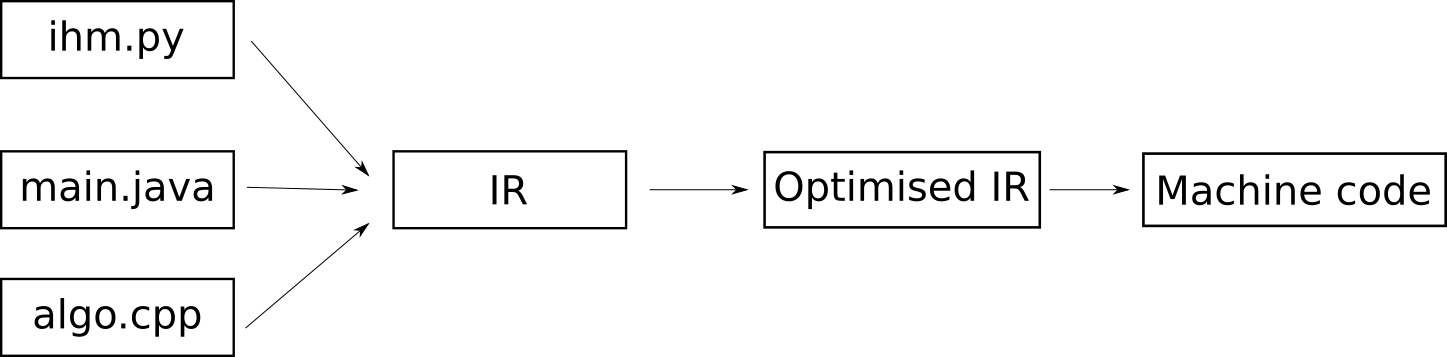
\includegraphics[scale=0.25]{gfx/LLVM/Architecture.png}
\caption{Simplified LLVM Architecture}
\label{fig:Architecture}
\end{figure}

On the left hand side, the input source file are processed by the front-ends corresponding to the language of the source code. The front-end provides to the rest of the pipeline a ll file, which is a file containing LLVM-IR. The tool use for the front end differ according to source code. For example, in case of C/C++, the tool can be clang.

These files are given to an optimiser and are optimized independently. A set of common optimisations can be performed. But the user can specify which passes to run. The tool for this stage is llvm-opt. It is possible to specify with an option to execute only some passes. For instance, to enable Polly, the "-polly" option is needed to allow polyhedral optimizations.

After this stage, llvm-link links every ll files into a single module.

This module can be optimized again with llvm-opt. All source code are merged in one module, so it is possible to optimise C++ code that is inside a python method. 

Once the ll file is optimized, an object file is generated using llvm-llc and llvm-mc. During these steps, optimizations for specific architectures can be done. For instance, generating instructions that handle array will not be generated in the same manner on a x86-64 processor and on a GPU.

\section{LLVM IR}
One of the best concept of LLVM is the intermediate representation. This language is used throughout all the LLVM Pipeline. Every compiler that uses LLVM as backend to optimize the code transforms the source code to a LLVM-IR version. LLVM-IR is independant of the target architecture, typed and assume an infinite number of registers. Each register is written only once so that the operations are in Static Single Assignement form (SSA). 

A LLVM-IR file is just a list of instructions. Passes can add, remove or modify instructions. For instance, it is possible to add malloc and free calls with the following methods :
\begin{lstlisting}[frame=single]
CreateMalloc (Instruction *InsertBefore, Type *IntPtrTy, Type *AllocTy, Value *AllocSize, Value *ArraySize=nullptr, Function *MallocF=nullptr, const Twine &Name="")
CreateFree (Value *Source, Instruction *InsertBefore)
\end{lstlisting}

In this thesis, some examples will be written in LLVM-IR for the sake of simplicity. If the reader has some troubles to understand the code, a full definition can be found here. \todo{add link}

\section{Passes}
LLVM works with a mechanism of passes. Passes perform transformations and optimizations on the code. They also make analysis that will be used by other passes. A pass can depends on others passes. For instance, a pass that get rid of dependencies will depend on the pass that computes these dependencies.

Each pass is register to a pass manager. It is possible to enable a pass in the opt command line by adding -<name of the pass>. 

There are multiples types of passes in LLVM, depending on which kind of object it iterate on. Here are the main one :
\begin{itemize}
\item ModulePass
\item FunctionPass
\item LoopPass
\item RegionPass
\item BasicBlockPass
\end{itemize}
A basic block is a single entry single exit section of code.

%************************************************
\chapter{Polly}\label{ch:Polly}
%************************************************

\section{Architecture}
Polly is a loop and data-locality optimizer for LLVM\cite{Polly}. The optimisations are made using a mathematical model called the polyhedral model. A key aspect of the model is the ability to reason about the memory access behavior in a very fine-granular way. This enables us to express very fine-granular way in a mathematical domain, where we deal with polyhedra instead of LLVM instructions. After modeling, transformations (tilling, loop fusion, loop unrolling …) can be applied on the model to improve data-locality and/or parallelization.

To do this, polly acts in three steps. First, it detects interesting code and translates it into a polyhedral representation. Then, it does some analysis and transformations passes that operate on the LLVM-IR. Finally, it generates code for the desired target. These three steps are called front-end, middle part and back-end passes. This pipeline is described in Figure~\ref{fig:Architecture}.

\begin{figure}
\centering
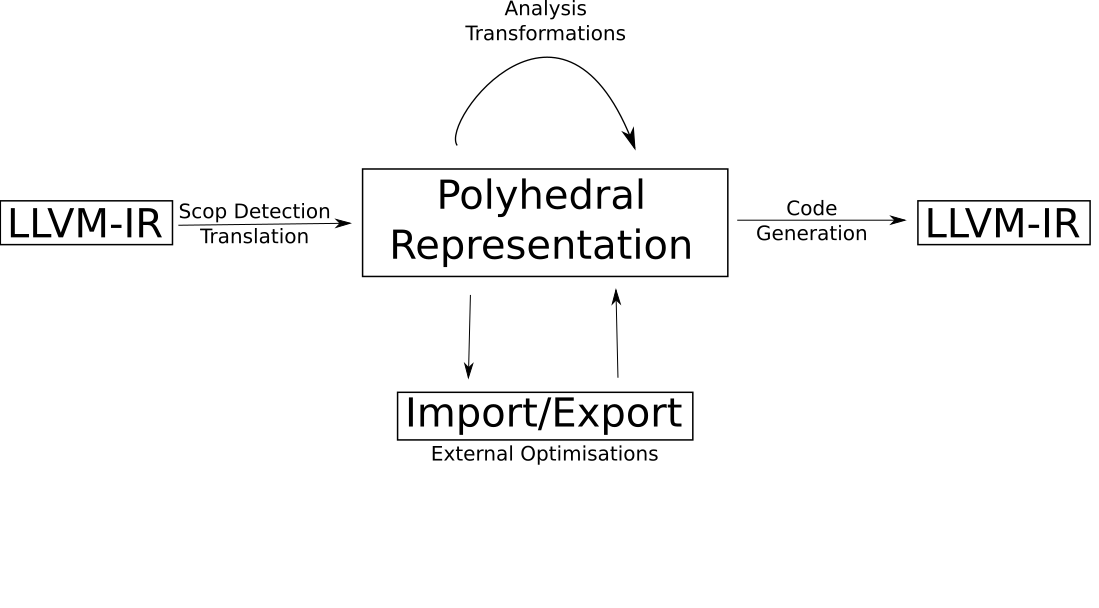
\includegraphics[scale=0.4]{gfx/Polly/Architecture.png}
\caption{Architecture of Polly}
\label{fig:PollyArchitecture}
\end{figure}

In the front-end passes, Polly detects which part of the code will be optimised. Those part are called \ac{SCOP}. Then Polly transforms those SCoPs into a polyhedral representation. 

The middle part is the place where analysis (dependencies analysis) and transformations (Maximal static expansion for instance) are made. It is also possible to export and import representations to perform manual optimisations.

Finally, in the back-end, the optimised polyhedral representation is transform back to LLVM-IR. It is possible to detect code that will take advantages of a thread level parallelism (OpenMP) and that will behave better with SIMD instructions. It is also possible to generate code for GPU. 

There are two ways to enable polly. It is possible to enable Polly directly from clang by adding the option \emph{-polly} to the clang command line. Multiple passes can be enable by just calling them from the command line. The resulting executable will then be an executable optimised with Polly. It is also possible to do it by hand with the LLVM tools seen in the preeceeding chapter.

\section{Profitable code and SCop}
Polly operates on a low level representation of the code called LLVM-IR. This language has been designed to perform low-level optimisations. To focus on important high-level optimisation problems, it is important to have a more abstract representation. In this section, we will discuss about the polyhedral representation used by Polly and a definition of what kind of code can be translated to this representation.

Polyhedral optimisers work on Static Control Parts (SCoP) of a function. A Static Control Parts is a part of code in which all control flow and memory accesses are known at compile time. This means that it is possible to run precise and detailled analysis during compilation. Some optimisers also work with non-statically known control flow, some use a \ac{JIT} mechanism, but Polly only focus on statically known control flow. An extension to Polly, called PolyJit\cite{PolyJit}, is able to operates at run-time.

\begin{definition}{}
A SCoP is a part of a code in which :
The control flow contains only for-loops and if-conditions and :
\begin{itemize}
\item Each loop has only one integer induction variable that is incremented between a lower and an upper bound, by a constant stride.
\item Lower and upper bounds are affine expressions in parameters and surrounding loop induction variables. A parameter is a integer variable that is keep constant throughout the SCoP.
\item If-conditions compare two affine expressions.
\item Statements inside for loops or if body are valid if and only if they are assignements that store an expression to an array element.
\item The access function consists of a formula with induction variables, parameters.
\item The expression stored can be a formula or a function call with inductions variables, parameters or array elements.
\end{itemize}\end{definition}

Polly, by default, does not optimise all SCoPs. It select profitable one with a very simple algorithm. A SCoP is considered profitable if :
\begin{itemize}
\item There are read and write statements.
\item There are at least two affine loops. 
\item There are more instruction per loop than a threshold.
\end{itemize}

It is possible to force Polly to optimise every SCoP with the option $-polly-process-unprofitable$. This approach is very simple and not efficient. During my thesis, one of my colleague has worked on a different approach to select profitable SCoP based on Profiled Guided Optimisation (PGO)\cite{PGO}.

After Scop transformations, Polly create a divergence at the place where the SCoP was. One branch is the old code, one other is the optimised version. Some tests, at runtime, are performed to choose the right code to be optimised. For instance, Polly is not able to handle pointers that overlapsed, but the detection can only be made at run-time. For a more visual understanding, see Figure~\ref{fig:ScopSplit}.
\begin{figure}
\centering
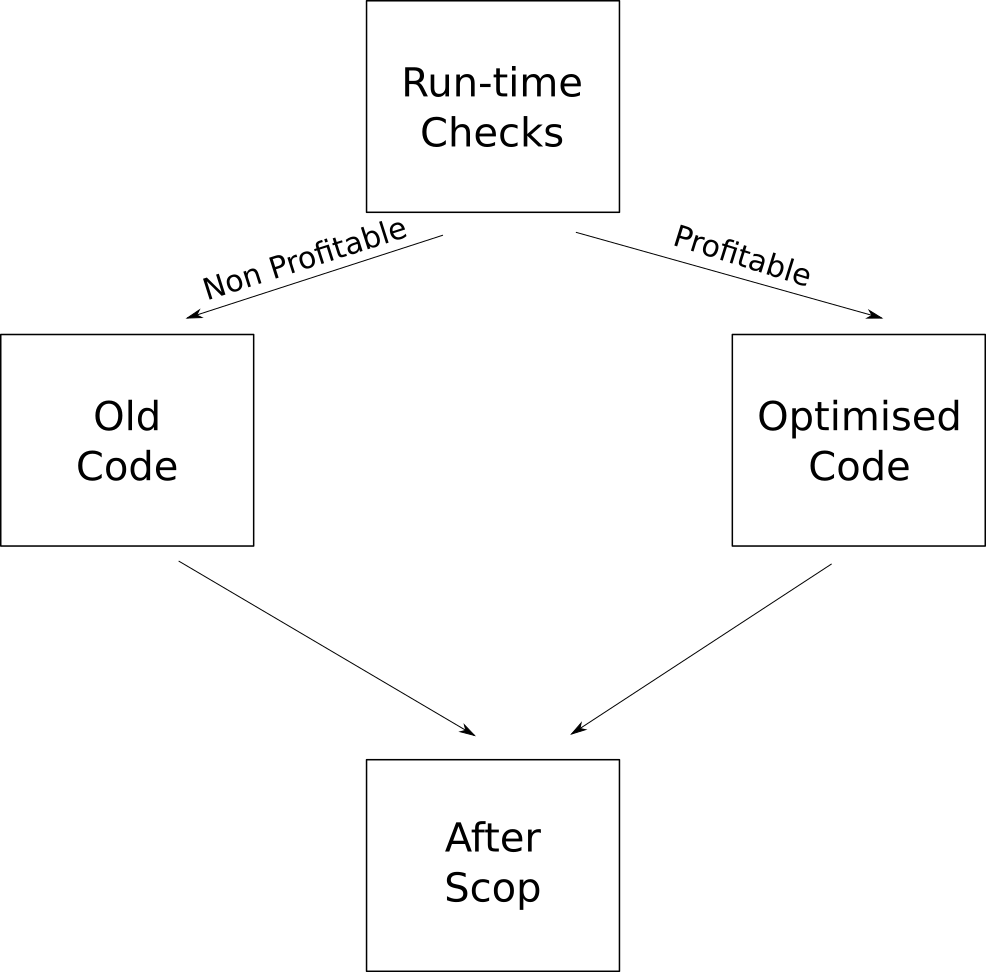
\includegraphics[scale=0.3]{gfx/Polly/ScopSplit.png}
\caption{Divergence between old code and new code}
\label{fig:ScopSplit}
\end{figure}


\section{Polyhedral representation inside Polly}
Polly uses a polyhedral representation based on ISL, the library described in chapter\ref{ch:ISL}.

A SCoP is described as a \emph{context} and a \emph{list of statements}. A \emph{context} is a set that describes constraints on parameters : positiveness, interval constraints, etc.

A \emph{statement} is a \emph{name}, a \emph{domain}, a \emph{schedule} and a list of \emph{accesses}. It represents the smallest unit that can be scheduled independantly.

A \emph{domain} is a named integer set that described the loops iterations. The name of the domain is the name of the statement it appears in. A domain has as many parameter dimensions as number of parameters of the SCoP. For each loop in the loop nest, the statement has one set dimension.

A \emph{schedule} is a map that assigns to each iteration vector, a point in time. This map is used to describe execution order of the statements instances.

A \emph{access} is a \emph{kind} and a \emph{relation}. The \emph{kind} can be $write$, $read$ or $MayWrite$. $MayWrite$ occurs when the write access can be executed or not, depending on execution : a write access inside a if-condition is represented as a $MayWrite$. A \emph{relation} is a map that maps statement domain to a memory location. 

To have a more clear view of the polyhedral representation, here is an example :
\begin{lstlisting}[frame=single]
for (int i = 0; i < N; i++) {
   for (int j = 0; j < N; j++) {
S:   B[i][j] = i*j;;
   }
}
\end{lstlisting}
There is only one statement in this \emph{SCoP}, named S.

The \emph{context} of this SCoP is :
\[
[N] -> \{ \}
\]

The \emph{domain} of S is :
\[
[N] -> \{ S[i][j] : 0\le i \le N \wedge 0\le j \le N \}
\]

There is only one memory access, a Write memory access, models as follows :
\[
\{ S[i][j] \rightarrow B[i][j] \}
\]

Polly also uses a ISL-based representation for dependences. An example can be found in chapter\ref{ch:ISL}.

\section{JSON Importer/Exporter}
Polly allows the user to export the SCoP representation into a JSON file. At the beginning, Polly was not able to perform optimisation. The aim of the JSON Importer/Exporter was to allow users to use their own polyhedral optimisers. 

Let take an example.
\begin{lstlisting}[frame=single]
int Ni = 1056;
int Nk = 1024;
int Nj = 1056;
void func(double beta, double A[Ni][Nk], double B[Ni][Nj]) {
  int i,j,k;

  for (i = 0; i < Ni; i++) {
    for (j = 0; j < Nj; j++) {
      for (k = 0; k < Nk; ++k) {
        B[i][j] = 10 * A[i][k];
      }
    }
  }
}
\end{lstlisting}

The JSCoP representation of this SCoP is :
\begin{lstlisting}[frame=single]
{
   "arrays" : [
      {
         "name" : "MemRef_A",
         "sizes" : [ "*", "1024" ],
         "type" : "double"
      },
      {
         "name" : "MemRef_B",
         "sizes" : [ "*", "1056" ],
         "type" : "double"
      }
   ],
   "context" : "{  :  }",
   "name" : "%for.cond1.preheader---%for.end18",
   "statements" : [
      {
         "accesses" : [
            {
               "kind" : "read",
               "relation" : "{ S[i0, i1, i2] -> MemRef_A[i0, i2] }"
            },
            {
               "kind" : "write",
               "relation" : "{ S[i0, i1, i2] -> MemRef_B[i0, i1] }"
            }
            }
         ],
         "domain" : "{ S[i0, i1, i2] : 0 <= i0 <= 1055 and 0 <= i1 <= 1055 and 0 <= i2 <= 1023 }",
         "name" : "S",
         "schedule" : "{ S[i0, i1, i2] -> [i0, i1, i2] }"
      }
   ]
}
\end{lstlisting}

As first step in open source software development and to get familiar with Polly/LLVM development process, I fixed an open bug in Polly. From a JSON file it is possible to alter the existing modelling of a SCoP and even trigger code generation for new array accesses. This interface is mainly used for debugging and testing and therefore lacked a lot of consistency checks. This often triggered errors in the remaining part of the Polly optimization pipeline. My first step was, therefore, to implement those missing checks.

The resulting commit can be found here at \footurl{https://reviews.llvm.org/D32739}{this link}.

\part{Implementation}
%************************************************
\chapter{Array Heap Allocation}\label{ch:HeapAlloc}
%************************************************

When doing the expansion, we need to create and allocate new arrays. Polly was already able to generate necessary array creation code, if that array has to be located on the stack as part of the pattern-based optimization of matrix multiplication. However, array allocation on the heap, which provides the amount of memory needed for full static array expansion was not possible before.

Consider the following code as an example:
\begin{lstlisting}[frame=single]
for (int i = 0; i < N; i++)
  for (int j = 0; j < N; j++)
    for (int k = 0; k < N; k++)
      for (int l = 0; l < N; l++)
        A[l] = 3;
\end{lstlisting}

The expansion would lead to the following code :
\begin{lstlisting}[frame=single]
for (int i = 0; i < N; i++)
  for (int j = 0; j < N; j++)
    for (int k = 0; k < N; k++)
      for (int l = 0; l < N; l++)
        A_exp[i][j][k][l] = 3;
\end{lstlisting}

Depending on the value of N, $A_{exp}$ can have a huge number of elements. If N = 100, we have $100*100*100*100 = 100000000 = 10^8$ elements ! Thus, the possibility to allocate array on heap was needed.

On the implementation side, special care had to be taken to get the memory allocation/deallocation correct. As opposed to stack-arrays which get freed automatically, heap allocated arrays require explicit calls to malloc and free. As Polly already guards the code that is generated during the execution of its’ optimization pipeline behind a branch, we have chosen to specifically create BasicBlocks right after the branch and right before the join to place our calls to malloc and free for any array that needed to be created on the heap. These two blocks can be seen on Figure~\ref{fig:HeapAllocPlace}.

\begin{figure}
\centering
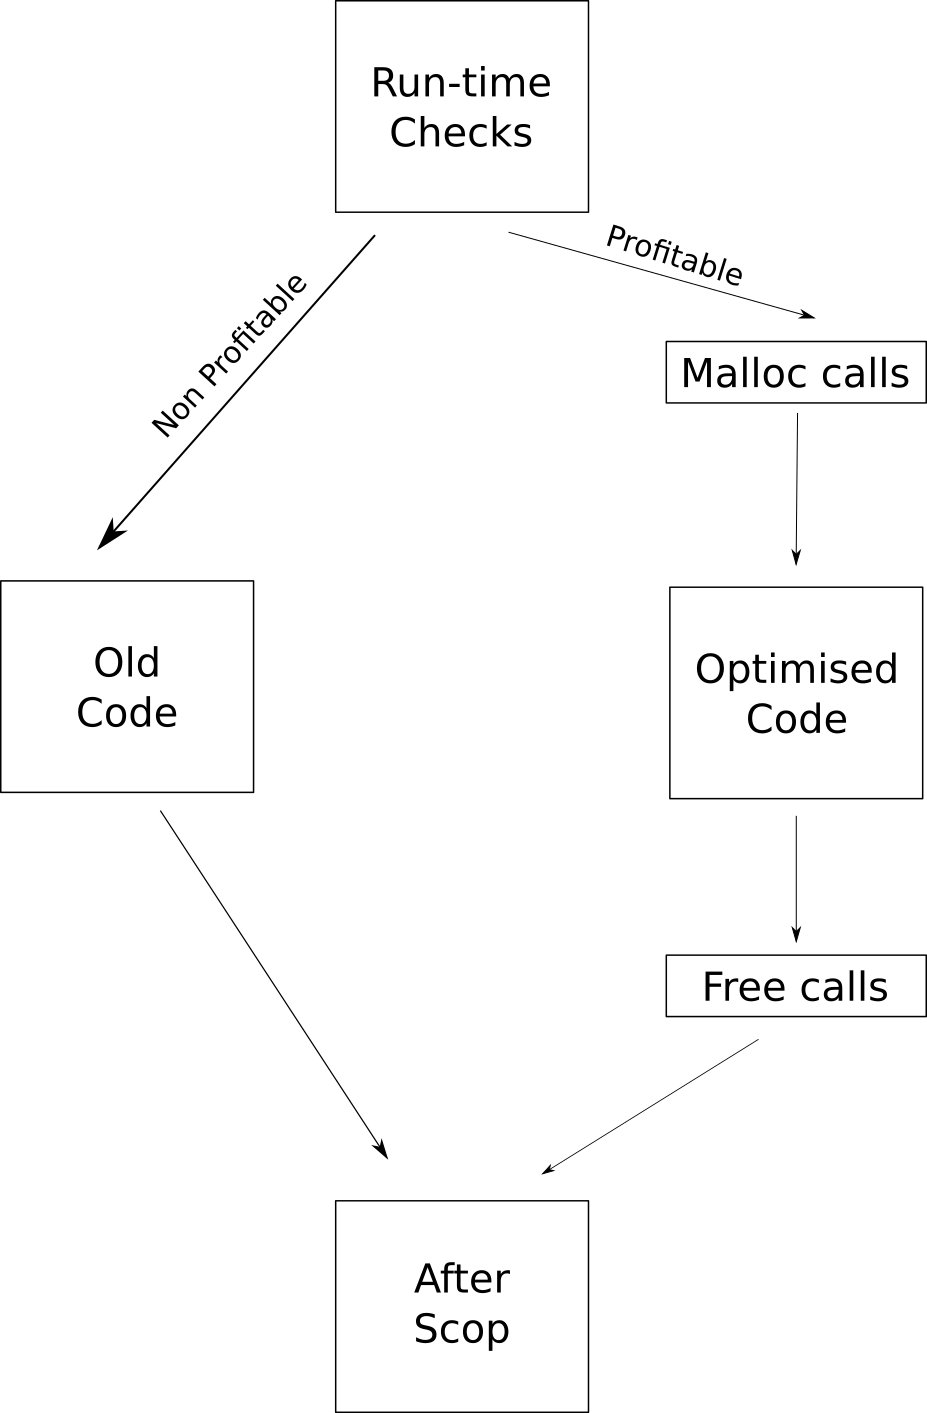
\includegraphics[scale=0.3]{gfx/HeapAlloc/ScopSplit.png}
\caption{Malloc/Free block positions}
\label{fig:HeapAllocPlace}
\end{figure}

As an incremental step, this could be tested via the JSON Importer. We concluded to this solution after long discussion with the Polly community to ensure that we do not risk a use after free error with the newly added arrays. Even if the SCoP is inside a loop, every allocated arrays we'll be freed. This solution is simple to implement but need a mechanism of copy-in/out. This problem will be discussed in a future section\todo{faire le lien}.

Technically speaking, to insert malloc and free calls, we used the method described in section\todo{add the link}. Here is a simplified version of the code actually in place :
\begin{lstlisting}[frame=single]
// Get the IntPtrTy from the Datalayout
auto IntPtrTy = DL.getIntPtrType(Ctx);

// Get the size of the element type in bits
unsigned Size = SAI->getElemSizeInBytes();

// Insert the malloc call at polly.start
auto InstIt = std::get<0>(StartExitBlocks)->getTerminator();
auto *CreatedArray = CallInst::CreateMalloc(
          &*InstIt, IntPtrTy, SAI->getElementType(),
          ConstantInt::get(Type::getInt64Ty(Ctx), Size),
          ConstantInt::get(Type::getInt64Ty(Ctx), ArraySizeInt), nullptr,
          SAI->getName());

SAI->setBasePtr(CreatedArray);

// Insert the free call at polly.exiting
CallInst::CreateFree(CreatedArray,
          std::get<1>(StartExitBlocks)->getTerminator());
\end{lstlisting}
Polly.start and Polly.exiting are respectively the first and the last BasicBlock of the Polly branch. These two BasicBlock are passed to this section of code via the pair \emph{StartExitBlocks}.
First, we create the malloc call :
\begin{lstlisting}[frame=single]
// Get the IntPtrTy from the Datalayout
auto IntPtrTy = DL.getIntPtrType(Ctx);

// Get the size of the element type in bits
unsigned Size = SAI->getElemSizeInBytes();

// Insert the malloc call at polly.start
auto InstIt = std::get<0>(StartExitBlocks)->getTerminator();
auto *CreatedArray = CallInst::CreateMalloc(
          &*InstIt, IntPtrTy, SAI->getElementType(),
          ConstantInt::get(Type::getInt64Ty(Ctx), Size),
          ConstantInt::get(Type::getInt64Ty(Ctx), ArraySizeInt), nullptr,
          SAI->getName());
\end{lstlisting}
There are multiple parameters but this call is pretty easy. The first parameter is the instruction before which to insert the call. The second is the type of a int pointer on the machine, we take the one from the DataLayout, a structure containing information about target. The next one is the type of element in the array. The 4th and 5th parameters are the size of one element and the total size of the array (product of all dimensions).

The free call is even more simple :
\begin{lstlisting}[frame=single]
// Insert the free call at polly.exiting
CallInst::CreateFree(CreatedArray,
          std::get<1>(StartExitBlocks)->getTerminator());
\end{lstlisting}
We get from CreateMalloc a pointer to the allocated memory. The CreateFree method take this pointer and the location where to insert the free. And that's all !

The finished support for heap allocation was committed into Polly and all discussion about it can be found \href{https://reviews.llvm.org/D33688}{here}.
%************************************************
\chapter{Full Index Expansion}\label{ch:FIE}
%************************************************
Maximal refers to a static expansion that requires the least amount of memory. As before, we have chosen an iterative approach to implement this. With the heap allocation and stable testing support in the JSONImporter in place, we proceed to implementing just any expansion and continue with the implementation of the maximal one. This ensures that we first focus on the correctness of the basic expansion. This will already provide us the elimination of all but true dependencies (also known as flow dependencies). Any optimization we apply afterwards will provide us with less space requirement and, therefore, only expand the useability in terms of memory consumption.

\section{Array expansion}
This will describe the most simple form of static expansion. From all possible memory access types (Scalars, Arrays, PHI) we have started with an implementation that supports the expansion of only arrays, because we only have to convert one array to another one. As a basic property of static expansion we have one single write per array cell. We ensure this by transforming each write-access into a new array (located on the heap). Afterwards, we have to remap all read accesses to the old write-access to the correct new array and the correct new array index (based on polyhedral dependency information). Naturally we would resort to statement-level dependencies, which map statement instances (i.e., “S[i][j]” in the example below) to statement- instances. However, due to the coarse granularity of polly (i.e., one BasicBlock forms one statement), we are forced to use reference-based dependencies. These give us the possibility to filter all dependencies for only the one array access that we are interested in for the expansion. The basic implementation of our Fully-Indexed Static Expansion was committed to Polly and can be found \footurl{https://reviews.llvm.org/D34982}{here}. The switch from Statement-Level to Reference-Level dependencies can be found \footurl{https://reviews.llvm.org/D36791}{here}.

\section{Scalar and PHI expansion}
Inside Polly one encounters scalar values of two kinds. First, the standard scalar value, which is just a single value (MemoryKind::Value). Second, a PHI node (MemoryKind::PHI). These virtual nodes are represented in Polly as scalar values that are read at the definition of the PHI node, and written at the end of every source BasicBlock. Let us consider the following example:

\begin{lstlisting}[frame=single]
int tmp = 0;
for (int i = 0; i < N; i++) {
    tmp = tmp + 2;
}
\end{lstlisting}

In LLVM, everything is transformed in SSA. This means that Polly sees the following source code :

\begin{lstlisting}[frame=single]
int tmp = 0;
for (int i = 0; i < N; i++) {
    tmp_1 = PHI(tmp, tmp_2)
    tmp_2 = tmp_1 + 2;
}
\end{lstlisting}

$tpm1$ has not always the same source depending on the iteration the i-loop is in. If i=0, the source is tmp otherwise the source is $tmp_2$ of the previous iteration.

The expansion of the scalar write access is trivial because it behaves similar to the array case. PHI nodes have to be treated a little bit different to normal memory accesses. Due to their nature of (guaranteed) one read and possibly multiple writes we can switch the roles and perform the same expansion as in the case of normal scalar values. The expansion to Scalars and PHI nodes was committed as well and can be found \footurl{https://reviews.llvm.org/D36647}{here}.

\section{Implementation details}
\subsection{runOnScop}
Let have a closer look to the algorithm behind expansion. Static expansion is done in a Scop Pass : a Pass that is executed on every Scop. A Scop Pass has a "main" method called runOnScop. Here is a simplified version of the runOnScop of static expansion pass.

\begin{lstlisting}[frame=single]
bool MaximalStaticExpander::runOnScop(Scop &S) {

  // Get the RAW Dependences.
  auto &DI = getAnalysis<DependenceInfo>();
  auto &D = DI.getDependences(Dependences::AL_Reference);
  auto Dependences = isl::give(D.getDependences(Dependences::TYPE_RAW));

  for (auto SAI : S.arrays()) {
    SmallPtrSet<MemoryAccess *, 4> AllWrites;
    SmallPtrSet<MemoryAccess *, 4> AllReads;
    if (!isExpandable(SAI, AllWrites, AllReads, S, Dependences))
      continue;

      auto TheWrite = *(AllWrites.begin());
      ScopArrayInfo *ExpandedArray = expandAccess(S, TheWrite);

      mapAccess(S, AllReads, Dependences, ExpandedArray, true);
    } else if (SAI->isPHIKind()) {
      expandPhi(S, SAI, Dependences);
    }
  }

  return false;
}
\end{lstlisting}

The first 3 lines is a way to get RAW dependencies from the DependenceInfo pass.

Then, we iterate over the ScopArrayInfo of the SCoP and try to expand this ScopArrayInfo.
\begin{itemize}
\item If the SAI is not expandable, we continue.
\item If the SAI is expandable, we expand the Write access and then we map the read accesses according to the algorithm detailed in Section~\ref{ch:MSE}.
\item If the access is a PHI access,  we expand the access with the same principle as before but the role of write and read are exchange.
\end{itemize}

\subsection{Write expansion}
We will described in this subsection how the write expansion is done inside Polly. An example will be runned throught the explanation. 
\begin{lstlisting}[frame=single]
for (int i=0; i<N; i++){
   for (int j=0; j<N; j++) {
S:    A[i] = 5;
   }
T: ... = A[i];
}
\end{lstlisting}

First we get the old write access relation.
\begin{lstlisting}[frame=single]
auto CurrentAccessMap = MA->getAccessRelation();
\end{lstlisting}
In our example :
\[
\{ S[i, j] \rightarrow A[i] : 0 \le i \le N, 0 \le j \le N\}
\]

Then, we create a new map with the same domain as the old relation.
\begin{lstlisting}[frame=single]
// Get domain from the current AM.
auto Domain = CurrentAccessMap.domain();

// Create a new AM from the domain.
auto NewAccessMap = isl::map::from_domain(Domain);
\end{lstlisting}
In our example :
\[
\{ S[i, j] \rightarrow [] : 0 \le i \le N, 0 \le j \le N\}
\]

We add out dimensions to this newly created map. We add one dimension per induction variable in the loop nest.
\begin{lstlisting}[frame=single]
unsigned in_dimensions = CurrentAccessMap.dim(isl::dim::in);

// Add dimensions to the new AM according to the current in_dim.
NewAccessMap = NewAccessMap.add_dims(isl::dim::out, in_dimensions);
\end{lstlisting}
In our example :
\[
\{ S[i, j] \rightarrow [o_1, 0_2] : 0 \le i \le N, 0 \le j \le N\}
\]

We create the new ScopArrayInfo and explicitly allocate this array on the heap.

\begin{lstlisting}[frame=single]
auto ExpandedSAI = S.createScopArrayInfo(ElementType, CurrentOutIdString, Sizes);
ExpandedSAI->setIsOnHeap(true);
\end{lstlisting}
Let say that the newly create ScopArrayInfo is called $A_exp$.

Then, we set the out id to the name of the newly created ScopArrayInfo.
\begin{lstlisting}[frame=single]
NewAccessMap = NewAccessMap.set_tuple_id(isl::dim::out, NewOutId);
\end{lstlisting}
In our example :
\[
\{ S[i, j] \rightarrow A_{exp}[o_1, 0_2] : 0 \le i \le N, 0 \le j \le N\}
\]

We have to add constraint to link the out and in dimensions, otherwise the relation is wrong.
\begin{lstlisting}[frame=single]
auto SpaceMap = NewAccessMap.get_space();
  auto ConstraintBasicMap =
      isl::basic_map::equal(SpaceMap, SpaceMap.dim(isl::dim::in));
  NewAccessMap = isl::map(ConstraintBasicMap);
\end{lstlisting}
In our example :
\[
\{ S[i, j] \rightarrow A_{exp}[o_1, 0_2] : 0 \le i \le N, 0 \le j \le N, i=o_1, j=o_2\}
\]
That can be simplified as :
\[
\{ S[i, j] \rightarrow A_{exp}[i, j] : 0 \le i \le N, 0 \le j \le N\}
\]

Finally we set the new access relation.
\begin{lstlisting}[frame=single]
MA->setNewAccessRelation(NewAccessMap);
\end{lstlisting}

The only-write expanded version of the code example is :
\begin{lstlisting}[frame=single]
for (int i=0; i<N; i++){
   for (int j=0; j<N; j++) {
S:    A_exp[i][j] = 5;
   }
T: ... = A[i];
}
\end{lstlisting}

\subsection{Read expansion}
Now that we have expanded the write, let do the read expansion ! The read expansion is just a remapping and is super easy.

In our example, the read access relation is :
\[
\{ T[i] \rightarrow A[i] : 0 \le i \le N\}
\]

The RAW dependency is :
\[
\{[T[i] \rightarrow A[i] \rightarrow [S[i,j] \rightarrow B[i,i]]:0<=i<=N,0<=j<=N\}
\]

First of all we get the current access relation.
\begin{lstlisting}[frame=single]
auto CurrentAccessMap = MA->getAccessRelation();
\end{lstlisting}
In our example :
\[
\{ T[i] \rightarrow A[i] : 0 \le i \le N\}
\]

Then, we intersect the set of RAW dependencies to get only those that are related to the memory access we want to expand.
\begin{lstlisting}[frame=single]
// Get RAW dependences for the current WA.
auto DomainSet = MA->getAccessRelation().domain();
auto Domain = isl::union_set(DomainSet);

// Get the dependences relevant for this MA.
isl::union_map MapDependences;
MapDependences = filterDependences(S, Dependences, MA);

auto NewAccessMap = isl::map::from_union_map(MapDependences);
\end{lstlisting}
Because we bailed out on case that cause us troubles, there should be only one left dependency. The method $filterDependences$ return this dependency as a Statement to Statement map.
In our example, the reference to reference dependency is :
\[
\{[T[i] \rightarrow A[i] \rightarrow [S[i,j] \rightarrow B[i,i]]:0<=i<=N,0<=j<=N\}
\]
So the corresponding statement to statement dependency is :
\[
\{T[i] \rightarrow S[i,j] : 0<=i<=N,0<=j<=N\}
\]

We replace the out id with the id of the newly created ScopArrayInfo.
\begin{lstlisting}[frame=single]
auto Id = ExpandedSAI->getBasePtrId();
NewAccessMap = NewAccessMap.set_tuple_id(isl::dim::out, Id);
\end{lstlisting}
In our example :
\[
\{T[i] \rightarrow A_{exp}[i,j] : 0<=i<=N,0<=j<=N\}
\]

Finally, we set the new access relation to the memory access.
\begin{lstlisting}[frame=single]
MA->setNewAccessRelation(NewAccessMap);
\end{lstlisting}

Finally, the expanded example is :
\begin{lstlisting}[frame=single]
for (int i=0; i<N; i++){
   for (int j=0; j<N; j++) {
S:    A_exp[i][j] = 5;
   }
T: ... = A_exp[i][i];
}
\end{lstlisting}

\section{Limitations}
\subsection{Read & Write access inside the same statement}
In the following we will describe a small limitation of our current implementation. Let us consider the following example :

\begin{lstlisting}[frame=single]
for (int i = 0; i < N; i++) {
    for (int j = 0; j < N; j++) {
        B[i] = ... ;
        ... = B[i];
    }
}
\end{lstlisting}

Polly will model the two instructions as one ScopStatement and detect two memory access inside this statement :

Read :
\[
\{ S[i, j] \rightarrow B[i] : 0 \le i \le N, 0 \le j \le N \}
\]

Write :
\[
\{ S[i, j] \rightarrow B[i] : 0 \le i \le N, 0 \le j \le N \}
\]  
    
Then Polly will give these two memory accesses to ISL. But ISL has no information on the order in which the memory accesses appear so it decide that the read comes first, which is not the case in our example. This is a design decision inside Polly that requires us to bail out if such a case is possible.

\subsection{Union map needed as access relation}
The setNewAccessRelation take as parameter a isl map. But some code may lead to union map as access relation. Let take us an example :

\begin{lstlisting}[frame=single]
for (int i = 0; i < N; i++) {
    B[i] = ... ;
    for (int j = 0; j < N; j++) {
        B[j] = ... ;
    }
    ... = B[i];
}
\end{lstlisting}

The only-write expanded version of this example would look like this :

\begin{lstlisting}[frame=single]
for (int i = 0; i < N; i++) {
    B_exp[i] = ... ;
    for (int j = o; j < M; j++) {
        B_exp2[i][j] = ... ;
    }
    ... = B[i+2];
}
\end{lstlisting}

To read of B can read either from $B_exp$ or from $B_exp2$. Its memory access relation would look like, assuming that $N>M$ :
\begin{gather}
\{ T[i] \rightarrow B\_exp[i] : i \ge M, 0 \le i \le N, 0 \le j \le M ;  \\
T[i] \rightarrow B\_exp2[i][i] : i < M, 0 \le i \le N, 0 \le j \le M \}
\end{gather}

This memory access relation is an union map. The method setNewAccessRelation does not take an union map but a map as parameter. Changing this would involve to much changes inside Polly. So we decided to bail out if the expansion would lead to an union map as access relation.

\subsection{Copy-In & Copy-Out}
For accesses that have been initialized outside the loop where we have our read statements, we need to be able to copy in any data that would have been read from the outside. Let us consider the following example:

\begin{lstlisting}[frame=single]
for (int i = 0; i < N; i++) {
    ... = B[i];
    for (int j = 0; j < N; j++) {
        B[j] = ... ;
    }
}
\end{lstlisting}

The expanded version of this example would look like :

\begin{lstlisting}[frame=single]
for (int i = 0; i < N; i++) {
    ... = B_exp[i][i];
    for (int j = 0; j < N; j++) {
        B_exp[i][j] = ... ;
    }
}

\end{lstlisting}

The problem is that nobody is writing Bexp[i][i] before it is reading. So we need a copy in mechanism to manually copy data to Bexp from the original array. This mechanism is not yet implemented. The same problem appears when someone is reading a value expanded outside of the Scop. This is the problem of copy-in/out. For now, we just bail out such cases.

Following our incremental approach we, therefore, preclude our expansion with aggressive filtering of all access patterns that we cannot handle yet (or not at all). This filtering will block the expansion of the memory access, if:
\begin{itemize}
\item the associated ScopArrayInfo performs a MayWrite access.
\item the associated ScopArrayInfo has more than one MustWrite access, because this would require us to form the union of more than one access and use it as the new access relation of the ScopArrayInfo. This is not supported by Polly for now.
\item we would have to read in data from the original array (Copy-In). This is still a work in progress and not yet supported. But nothing inside Polly prevents us in adding support for this.
\item we would have to read expanded data after the SCoP (Copy-Out). This is still a work in progress and not yet supported. But nothing inside Polly prevents us in adding support for this.
\item we find a read and a write access to the same array inside a single statement. Here we cannot guarantee correctness because of the granularity of statements inside Polly.


\end{itemize}

%************************************************
\chapter{Implementation of Maximal Static Expansion}\label{ch:MSEImp}
%************************************************


\cleardoublepage
\part{Evaluation}

\cleardoublepage
\part{Perspectives}

% ********************************************************************
% Backmatter
%*******************************************************
%\appendix
%%\renewcommand{\thechapter}{\alph{chapter}}
%\cleardoublepage
%\part{Appendix}
%%********************************************************************
% Appendix
%*******************************************************
% If problems with the headers: get headings in appendix etc. right
%\markboth{\spacedlowsmallcaps{Appendix}}{\spacedlowsmallcaps{Appendix}}
\chapter{Appendix Test}
Lorem ipsum at nusquam appellantur his, ut eos erant homero
concludaturque. Albucius appellantur deterruisset id eam, vivendum
partiendo dissentiet ei ius. Vis melius facilisis ea, sea id convenire
referrentur, takimata adolescens ex duo. Ei harum argumentum per. Eam
vidit exerci appetere ad, ut vel zzril intellegam interpretaris.
\graffito{More dummy text.}

%Errem omnium ea per, pro congue populo ornatus cu, ex qui dicant
%nemore melius. No pri diam iriure euismod. Graecis eleifend
%appellantur quo id. Id corpora inimicus nam, facer nonummy ne pro,
%kasd repudiandae ei mei. Mea menandri mediocrem dissentiet cu, ex
%nominati imperdiet nec, sea odio duis vocent ei. Tempor everti
%appareat cu ius, ridens audiam an qui, aliquid admodum conceptam ne
%qui. Vis ea melius nostrum, mel alienum euripidis eu.

\section{Appendix Section Test}
Test: \autoref{tab:moreexample} (This reference should have a 
lowercase, small caps \spacedlowsmallcaps{A} if the option 
\texttt{floatperchapter} is activated, just as in the table itself
 $\rightarrow$ however, this does not work at the moment.)

\begin{table}[h]
    \myfloatalign
  \begin{tabularx}{\textwidth}{Xll} \toprule
    \tableheadline{labitur bonorum pri no} & \tableheadline{que vista}
    & \tableheadline{human} \\ \midrule
    fastidii ea ius & germano &  demonstratea \\
    suscipit instructior & titulo & personas \\
    %postulant quo & westeuropee & sanctificatec \\
    \midrule
    quaestio philosophia & facto & demonstrated \\
    %autem vulputate ex & parola & romanic \\
    %usu mucius iisque & studio & sanctificatef \\
    \bottomrule
  \end{tabularx}
  \caption[Autem usu id]{Autem usu id.}
  \label{tab:moreexample}
\end{table}

%Nulla fastidii ea ius, exerci suscipit instructior te nam, in ullum
%postulant quo. Congue quaestio philosophia his at, sea odio autem
%vulputate ex. Cu usu mucius iisque voluptua. Sit maiorum propriae at,
%ea cum primis intellegat. Hinc cotidieque reprehendunt eu nec. Autem
%timeam deleniti usu id, in nec nibh altera.




\section{Another Appendix Section Test}
Equidem detraxit cu nam, vix eu delenit periculis. Eos ut vero
constituto, no vidit propriae complectitur sea. Diceret nonummy in
has, no qui eligendi recteque consetetur. Mel eu dictas suscipiantur,
et sed placerat oporteat. At ipsum electram mei, ad aeque atomorum
mea. There is also a useless Pascal listing below: \autoref{lst:useless}.

\begin{lstlisting}[float=b,language=Pascal,frame=tb,caption={A floating example (\texttt{listings} manual)},label=lst:useless]
for i:=maxint downto 0 do
begin
{ do nothing }
end;
\end{lstlisting}

%Ei solet nemore consectetuer nam. Ad eam porro impetus, te choro omnes
%evertitur mel. Molestie conclusionemque vel at, no qui omittam
%expetenda efficiendi. Eu quo nobis offendit, verterem scriptorem ne
%vix.




%********************************************************************
% Other Stuff in the Back
%*******************************************************
\cleardoublepage%********************************************************************
% Bibliography
%*******************************************************
% work-around to have small caps also here in the headline
\manualmark
\markboth{\spacedlowsmallcaps{\bibname}}{\spacedlowsmallcaps{\bibname}} % work-around to have small caps also
%\phantomsection 
\refstepcounter{dummy}
\addtocontents{toc}{\protect\vspace{\beforebibskip}} % to have the bib a bit from the rest in the toc
\addcontentsline{toc}{chapter}{\tocEntry{\bibname}}
\label{app:bibliography}
\printbibliography

%\cleardoublepage%*******************************************************
% Declaration
%*******************************************************
\refstepcounter{dummy}
\pdfbookmark[0]{Declaration}{declaration}
\chapter*{Declaration}
\thispagestyle{empty}
Put your declaration here.
\bigskip
 
\noindent\textit{\myLocation, \myTime}

\smallskip

\begin{flushright}
    \begin{tabular}{m{5cm}}
        \\ \hline
        \centering\myName \\
    \end{tabular}
\end{flushright}

%\cleardoublepage\pagestyle{empty}

\hfill

\vfill


\pdfbookmark[0]{Colophon}{colophon}
\section*{Colophon}
This document was typeset using the typographical look-and-feel \texttt{classicthesis} developed by Andr\'e Miede. 
The style was inspired by Robert Bringhurst's seminal book on typography ``\emph{The Elements of Typographic Style}''. 
\texttt{classicthesis} is available for both \LaTeX\ and \mLyX: 
\begin{center}
\url{https://bitbucket.org/amiede/classicthesis/}
\end{center}
Happy users of \texttt{classicthesis} usually send a real postcard to the author, a collection of postcards received so far is featured here: 
\begin{center}
\url{http://postcards.miede.de/}
\end{center}
 
\bigskip

\noindent\finalVersionString

%Hermann Zapf's \emph{Palatino} and \emph{Euler} type faces (Type~1 PostScript fonts \emph{URW
%Palladio L} and \emph{FPL}) are used. The ``typewriter'' text is typeset in \emph{Bera Mono}, 
%originally developed by Bitstream, Inc. as ``Bitstream Vera''. (Type~1 PostScript fonts were made 
%available by Malte Rosenau and
%Ulrich Dirr.)

%\paragraph{note:} The custom size of the textblock was calculated
%using the directions given by Mr. Bringhurst (pages 26--29 and
%175/176). 10~pt Palatino needs  133.21~pt for the string
%``abcdefghijklmnopqrstuvwxyz''. This yields a good line length between
%24--26~pc (288--312~pt). Using a ``\emph{double square textblock}''
%with a 1:2 ratio this results in a textblock of 312:624~pt (which
%includes the headline in this design). A good alternative would be the
%``\emph{golden section textblock}'' with a ratio of 1:1.62, here
%312:505.44~pt. For comparison, \texttt{DIV9} of the \texttt{typearea}
%package results in a line length of 389~pt (32.4~pc), which is by far
%too long. However, this information will only be of interest for
%hardcore pseudo-typographers like me.%
%
%To make your own calculations, use the following commands and look up
%the corresponding lengths in the book:
%\begin{verbatim}
%    \settowidth{\abcd}{abcdefghijklmnopqrstuvwxyz}
%    \the\abcd\ % prints the value of the length
%\end{verbatim}
%Please see the file \texttt{classicthesis.sty} for some precalculated 
%values for Palatino and Minion.
%
%    \settowidth{\abcd}{abcdefghijklmnopqrstuvwxyz}
%    \the\abcd\ % prints the value of the length





% ********************************************************************
% Game Over: Restore, Restart, or Quit?
%*******************************************************
\end{document}
% ********************************************************************
